\documentclass{article}
\usepackage{graphicx} % Required for inserting images
\usepackage[margin=2cm, top=3cm]{geometry} % margine superiore ridotto a 1 cm
\usepackage{listings}
\usepackage{subcaption}  % Pacchetto per sottodidascalie
\usepackage{float}       % Pacchetto per posizionamento rigido delle figure
\usepackage{xcolor} % Pacchetto per i colori
\usepackage{amsmath} % Pacchetto per simboli avanzati

\title{Sistemi Operativi Esame}
\author{Mattia Cosimi}
\date{January 2025}

\begin{document}

\maketitle

\section{Prima Lezione: Introduzione alla riga di comando}
\begin{figure}[H] % Usa 'H' per forzare la posizione qui
    \centering % Centra l'immagine
    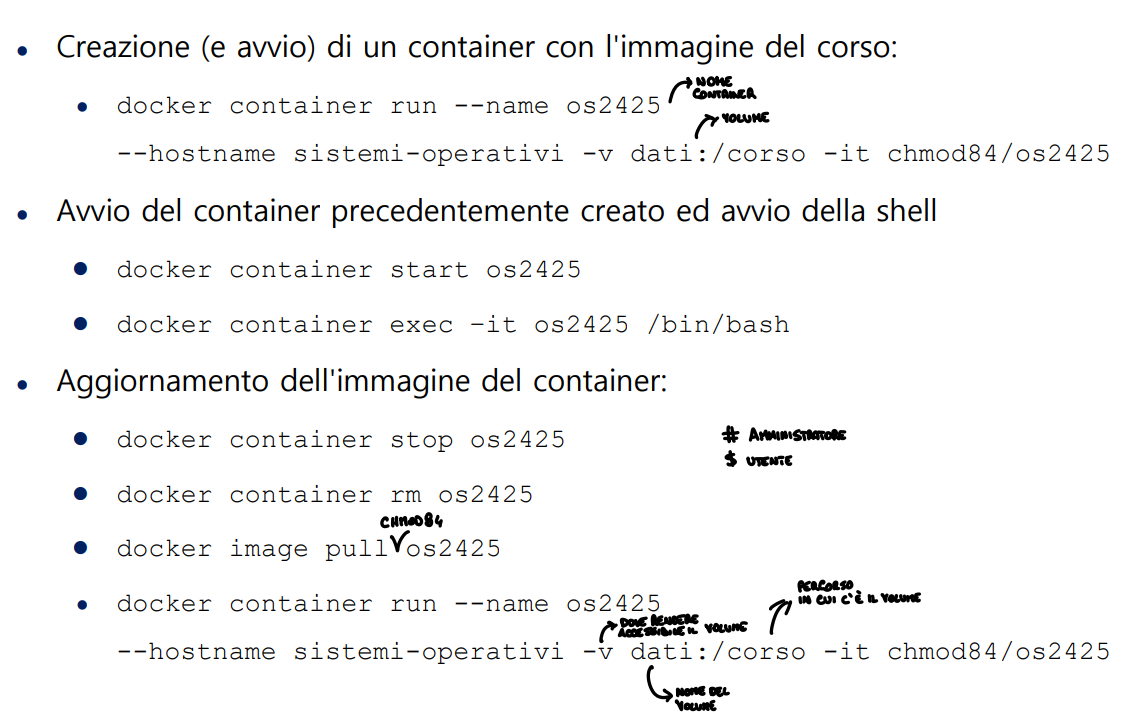
\includegraphics[width=16cm, height=10cm]{immagine_2025-01-22_123516228.png} % Percorso dell'immagine
   % \caption{Datagram Header} % Didascalia per l'immagine
    \label{fig:immagine} % Etichetta per riferimento
\end{figure}
\noindent
\subsection{Significato di quello che scriviamo/vediamo}
Se scriviamo \textbf{Docker} e premiamo invio mi fa vedere le varie azioni che posso fare, anche se eseguiamo \textbf{Docker container} ci da ulteriori suggerimenti. In \textbf{--name} possiamo mettere quello che vogliamo \textbf{--hostname} anche qui possiamo mettere quello che vogliamo sarebbe il nome della macchina, \textbf{-v} serve a specificare un nome di volume (\textbf{dati}), : dove vogliamo andare a rendere accessibile il volume di nome \textbf{dati}. \textbf{-it} serve a dire che il container che vogliamo creare deve essere "interattivo", a seguire il nome dell'immagine che ci voglio mettere dentro (una copia), avremmo potuto aggiungere :nome versione. Ora troveremo \textbf{corso@sistemi-operativi:\~\$} si chiama prompt. A sinistra della chiocciola c'è il \textbf{nome utente} che sta utilizzando il sistema (ogni utente ha permessi diversi). Invece sistemi-operativi è l'\textbf{hostname}. \textbf{Tilde} indica la cartella in cui ci troviamo in questo momento (percorso \textbf{home directory}), \textbf{Dollaro} è un indicatore che ci dice che dopo dobbiamo inserire i comandi (\textbf{Dollaro} utente, \textbf{Cancelletto} amministratore).\\\\
\subsection{Comandi}
\textbf{PWD (Print Working Directory)} stampa la cartella nella quale stiamo lavorando (working directory).\\\\
Quando lavoriamo con le cartelle, il percorso può avere uno \textbf{slash} finale se siamo di fronte a una cartella, se siamo di fronte a un \textbf{file} non lo avrà.\\\\
\textbf{CD (Change Directory)} mi permette di cambiare cartella, prende come argomento \textbf{il percorso dove vogliamo andare}. Se non gli diamo argomenti ci riporta nella \textbf{home directory} (directory di casa: possiamo fare tutto quello che vogliamo).\\\\
Esistono due percorsi, se iniziano con / allora sono \textbf{assoluti} sennò sono \textbf{relativi}. Gli \textbf{assoluti} identificano tutto il percorso da fare a partire dalla radice, i \textbf{relativi} vengono utilizzati da Linux concatenando la wd con il percorso relativo. \textbf{Importanti}: directory \textbf{.} identifica la directory corrente, la directory \textbf{..} rappresenta la directory superiore. Ovviamente si possono concatenare, es. \textbf{../../} ti porta indietro di due cartelle.\\\\
\textbf{MKDIR (Make Directory)} permette la creazione di una o più directory. L'argomento è un \textbf{percorso} che può essere relativo o assoluto. Per creare cartelle una dentro l'altra aggiungiamo \textbf{-p} (es. mkdir -p dir4/dir5/dir6)\\\\
\textbf{LS (List)} ci permette di vedere gli elementi della directory corrente. Si può inserire un argomento in modo tale da vedere il contenuto di quella directory.
\section{Seconda Lezione: Introduzione alla riga di comando}
\subsection{Gestione degli spazi}
Ci sono diversi modi: \textbf{utilizzo di " o '} (es. "folder 1"). Oppure l'utilizzo del carattere di escape (es. folder(backslash)3).
\subsection{Comandi (Gestione di un file)}
Si può redirigere l'output di un comando su file tramite l'operatore \textbf{$>$} (es. ls $>$ output.txt). \textbf{ATTENZIONE}: quest'operatore va a troncare il contenuto del file e riscriverlo, quindi se lo eseguo due volte il contenuto del file non si duplica.\\\\
Con l'operatore di ridirezione $>>$ questo problema si risolve\\\\
\textbf{CAT (Concatenate)} (copio il contenuto del file all'interno dello stdoutput) Questo comando oltre a stampare a video il contenuto del file, prende come argomenti i \textbf{file} che voglio stampare a video ("li concatena").\\\\
\textbf{ECHO} stampa sullo standard output quello che gli passo da riga di comando. (es. echo "Ciao sono Stefano" $>$ stefano.txt, ora il file stefano.txt verrà creato e avrà all'interno Ciao sono stefano).\\\\
\textbf{LESS} ci permette di vedere a schermo tutto il contenuto del file e scorrere con le freccette.\\\\
\textbf{MORE} ci permette di fare la stessa cosa di LESS "depotenziata". Per uscire dai comandi basta premere \textbf{Q}.\\\\
\textbf{MV (Move)} ci permette di spostare elementi all'interno del file system. (es. mv nomefile nomecartella/nomepercorso). Posso spostare più elementi basta che l'ultimo elemento della riga sia una cartella. Possiamo usarlo per \textbf{ridenominare} (es. mv combined.txt combined2.txt)\\\\
\textbf{CP (Copy)} ci permette di copiare un file. (es. cp nomefile percorso) è inoltre possibile copiare il contenuto dentro un altro file mettendo cp nomefile nome-file. (es. cp dir2/combined.txt ./combined-copia.txt crea nella directory corrente combined-copia.txt e mettici dentro il contenuto di combined.txt)\\\\
\textbf{RM (remove)} ci consente di eliminare i file (es. rm percorso/nomefile.txt).\\\\
\textbf{RMDIR (Remove diretory)} ci consente di eliminare le cartelle. Non funziona se la cartella ha qualcosa all'interno.\\\\
\textbf{RM} ha una versione ricorsiva, che va a togliere tutto il contenuto di una cartella. \textbf{RM -r }. Posso aggiungere \textbf{-v} per un livello di verbosità maggiore ovvero ci fa capire meglio cosa accade (in questo caso ci fa capire cosa va a cancellare).
\section{Terza Lezione: Introduzione alla riga di comando}
\subsection{Caratteri speciali}
Il carattere \textbf{speciale} $\ast$ serve a dire "sostituisci con zero o più caratteri qualunque. (Es: qualcosa$\ast$ corrisponde a tutte le stringhe che hanno qualcosa come prefisso) (Es: $\ast$qualcosa corrisponde a tutte le stringhe che hanno qualcosa come suffisso) (Es: $\ast$qualcosa$\ast$ corrisponde a tutte le stringhe che hanno al loro interno qualcosa)\\\\
Il carattere \textbf{speciale ?} vuol dire sostituisci un carattere solo. (Es. guarda $\ast$ solo che riempie con un solo carattere). \textbf{Entrambi} i caratteri non devono per forza comparire all'estremità della stringa.
\subsection{Comandi}
\textbf{WC (word count)}. \textbf{WC -l} Ci permette di contare le righe all'interno di un file. \textbf{WC -c} per contare il numero di caratteri. \textbf{WC} normale ci dice numeroRighe numeroDiParole numeroDiCaratteri. Se inserisco il comando \textbf{senza} nome di file, il sistema si aspetta un input da \textbf{stdinput}.\\\\
In questa lezione inoltre capiamo come mandare in input lo stream dello stdoutput.\\\\
\textbf{Operatore di Pipe $|$} ci consente di staccare stdout di un comando e mandarlo in input a un altro comando (es. ls $|$ wc).\\\\
\textbf{UNIQ} ci consente di contare il numero di righe uniche all'interno di (le righe identiche devono essere adiacenti) un file. Un esempio potrebbe essere: cat combined.txt $|$ uniq $|$ wc -l (stiamo chiedendo di mandare in input al comando uniq il cat di combined.txt che a sua volta manderà in input il numero di righe differenti a wc -l).\\\\
\textbf{SORT} ordina alfabeticamente il contenuto del file.
\section{Quarta lezione: Introduzione ai sistemi operativi}
Le \textbf{chiamate di sistema} hanno l'aspetto di funzioni che però non fanno parte di una libreria me bensì sono direttamente esposte dal nucleo del sistema operativo.
\subsection{Programma cpu.c}
\begin{figure}[H] % Usa 'H' per forzare la posizione qui
    \centering % Centra l'immagine
    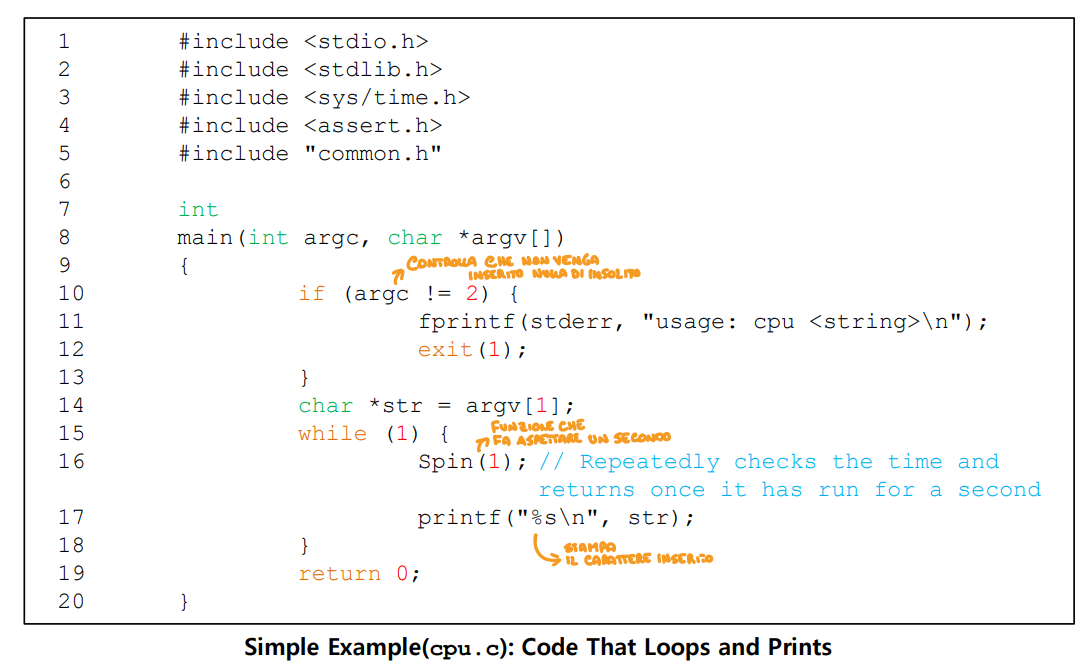
\includegraphics[width=16cm, height=10cm]{immagine_2025-01-22_194302712.png} % Percorso dell'immagine
   % \caption{Datagram Header} % Didascalia per l'immagine
    \label{fig:immagine} % Etichetta per riferimento
\end{figure}
\noindent
Si trova dentro ostep-code. Controlla se gli argomenti sono diversi da 2, in caso stampa una riga che dice guarda l'uso è una stringa. Dopodichè ogni secondo stampa una stringa. \textbf{ATTENZIONE}: non lasciare i file dentro ostep-code, vengono cancellati, lasciali dentro /home/corso.\\\\
\textbf{gcc -Wall -o cpu cpu.c} per la compilazione di un file (-Wall è opzionale).\\\\
Su windows se inserisco un nome di un file per eseguirlo lui di default lo va a cercare nella \textbf{working directory}, su linux non c'è quindi bisogna specificare \textbf{./cpu}\\\\
\textbf{TOP} ci consente di vedere varie informazioni, tra cui i processi (equivalente del task manager).\\\\
\textbf{\&} ci consente di mandare in background il comando che la precede e di mandare in esecuzione il comando che la succede. Per cancellare tutte le istanze di programmi \textbf{killall cpu}.
\subsection{Programma mem.c}
\begin{figure}[H] % Usa 'H' per forzare la posizione qui
    \centering % Centra l'immagine
    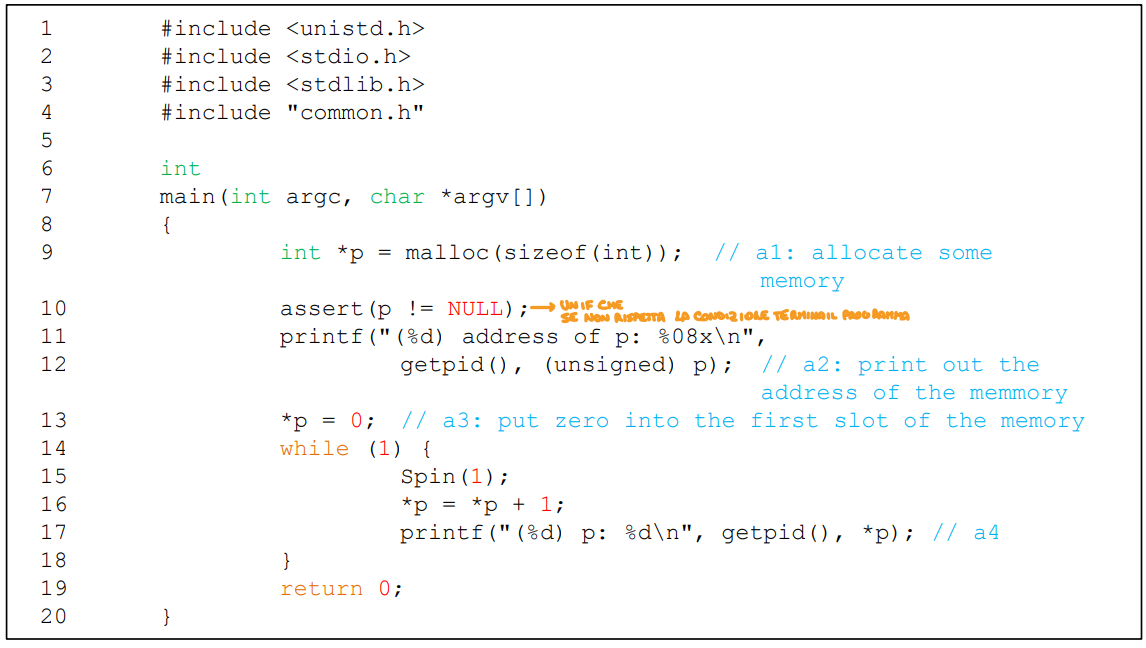
\includegraphics[width=17cm, height=10cm]{immagine_2025-01-23_104538610.png} % Percorso dell'immagine
   % \caption{Datagram Header} % Didascalia per l'immagine
    \label{fig:immagine} % Etichetta per riferimento
\end{figure}
\noindent
P è un puntatore a intero. \textbf{Assert} è un'istruzione in cui se quello che c'è tra parentesi non è soddisfatto il programma viene terminato. La prima \textbf{printf} dice: tra parentesi c'è un numero intero che viene sostituito dal \textbf{processId} (getPid()). Dopo address di p viene messo in \textbf{esadecimale} l'indirizzo del puntatore. Quindi ogni secondo quest'applicazione \textbf{aggiorna e incrementa} di 1 il valore di p. Sulla cartella ostep-code c'è una versione leggermente diversa con la funzione \textbf{atoi} che ci converte un numero scritto a caratteri e ci restituisce un intero.\\\\
\begin{figure}[H] % Usa 'H' per forzare la posizione qui
    \centering % Centra l'immagine
    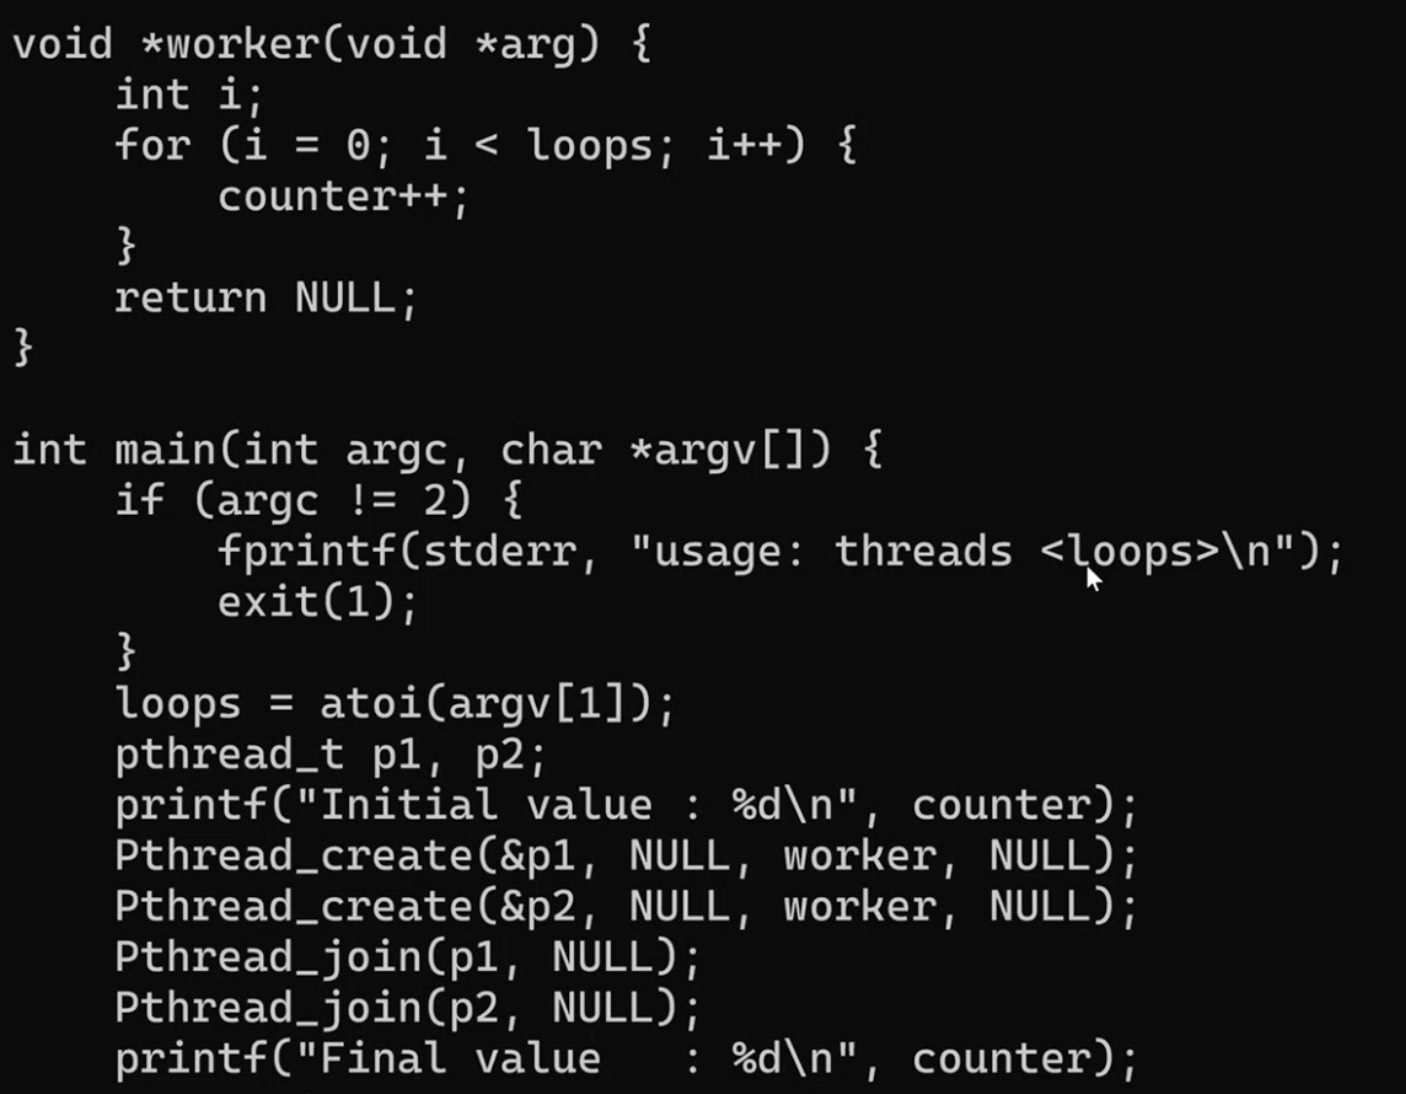
\includegraphics[width=17cm, height=8cm]{IMG_0842.jpeg} % Percorso dell'immagine
   % \caption{Datagram Header} % Didascalia per l'immagine
    \label{fig:immagine} % Etichetta per riferimento
\end{figure}
\noindent
Ora viene analizzata \textbf{threads.c}. Inizialmente chiama una variabile counter e la imposta a 0 (non presente nell'immagine) e una variabile globale loops. Oltre al main abbiamo un'altra funzione chiamata \textbf{worker}, la quale incrementa counter loops volte di uno. Per quanto riguarda il main, di nuovo vi è l'utilizzo dei \textbf{thread}. Immaginiamo che fino ad oggi abbiamo scritto le applicazioni con un unico filo di esecuzione (può utilizzare al più un core alla volta), vediamo ora un'applicazione con più fili e che quindi può utilizzare più core contemporaneamente. \\\\
\textbf{$pthread\_t$} dichiaro due thread e li creo con \textbf{$pthread\_create$}, i quali andranno a eseguire la funzione chiamata worker. Quindi attendiamo che il primo thread termini, attendiamo che il secondo termini e poi andiamo a stampare il valore di counter.
\subsubsection{Problema di Thread.c}
Ci aspettiamo che il valore di counter venga raddoppiato rispetto al numero di \textbf{loops} (essendo due i thread), questo però non funziona per valori molto grandi, quello che noi pensiamo essere un'istruzione su una riga (counter++), in realtà richiede che: counter= significa andare a scrivere qualcosa dentro counter, 1 istruzione, a destra c'è counter+1 che significa, accedi alla memoria leggi il valore di counter incrementalo e scrivi dentro counter il risultato. Le tre istruzioni non vengono eseguite in modo \textbf{atomico}. Cosa succede? i thread cercano contemporaneamente di aggiornare counter, il sistema operativo che assegna una porzione di tempo per ogni cpu, interrompe un processo ne fa continuare un'altro ecc... (es. il primo thread legge il valore di counter, vede che è 10, in questo momento il sistema operativo dice ok non è più il tuo turno è il turno dell'altro thread, il quale legge il valore di thread (10) somma uno e lo rimette in counter quindi counter ora è 11, continuo finchè non mi interrompe il sistema operativo, magari sono arrivato a 450, ora il sistema operativo ridà il controllo al primo thread il quale aveva appena letto 10 ora va a fare +1 e quindi counter sarà uguale a 11. ecco perchè il valore di counter sarà minore della somma dei loop). Per valori molto bassi funziona perchè i thread hanno lavorato in modo \textbf{sequenziale}.
\subsection{Programma io.c (Persistenza)}
\begin{figure}[H] % Usa 'H' per forzare la posizione qui
    \centering % Centra l'immagine
    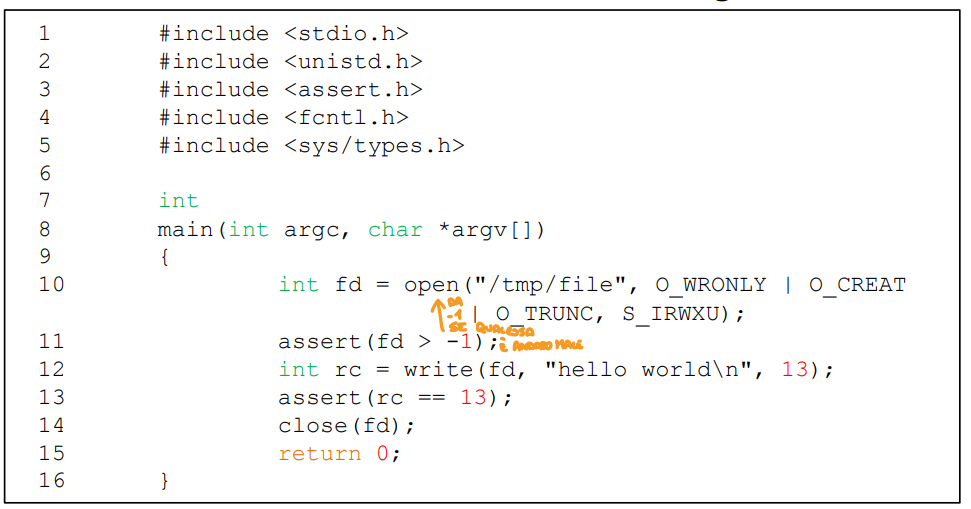
\includegraphics[width=17cm, height=8cm]{immagine_2025-01-23_113535172.png} % Percorso dell'immagine
   % \caption{Datagram Header} % Didascalia per l'immagine
    \label{fig:immagine} % Etichetta per riferimento
\end{figure}
\noindent
Questo programma tramite la chiamata di sistema \textbf{open} va a aprire un file che si trova nel percorso /tmp/file. Per quanto riguarda i parametri a sinistra della open, sono dei "permessi", \textbf{wronly} (apertura del file di sola scrittura), \textbf{creat} (se il file che ti ho specificato nel percorso non esiste crealo), \textbf{trunc} (se il file dovesse esistere troncalo), la assert ha lo stesso scopo di prima. La chiamata \textbf{write} scrive nel file specificato, il tredici alla fine consiste nella lunghezza della stringa hello world (n. byte). La \textbf{write} ci ritorna il numero di caratteri scritti nel file (13).
\section{Quinta lezione: process API}
\subsection{Scrittura di un file (editor)}
Quando voglio andare a scrivere un file ho due modi: il primo crearlo all'interno del container utilizzando un editor di testo \textbf{"da riga di comando"} oppure utilizzare un editor di testo \textbf{qualsiasi} e copiare il file all'interno del container per andarlo a compilare.\\\\
\textbf{NANO} (nano nomefiledacreare.c) è l'editor di testo da riga di comando. Ci illumina la sintassi. Per \textbf{salvare} ctrl+O - invio. Per \textbf{uscire} ctrl+X.\\\\
Per il secondo metodo, apriamo l'editor di testo e scriviamo il codice. Per \textbf{portarlo all'interno del container} scriviamo \textbf{docker cp} (nomeFile) nomeContainer:/percorso.\\\\
Il professore suggerisce di copiare la cartella ostep-code in /home/corso in modo tale da non perderne il contenuto quando andiamo a aggioranre l'immagine. \textbf{cp -r nomeCartella Percorso}.
\subsection{Chiamata di sistema: Fork()}
\begin{figure}[H] % Usa 'H' per forzare la posizione qui
    \centering % Centra l'immagine
    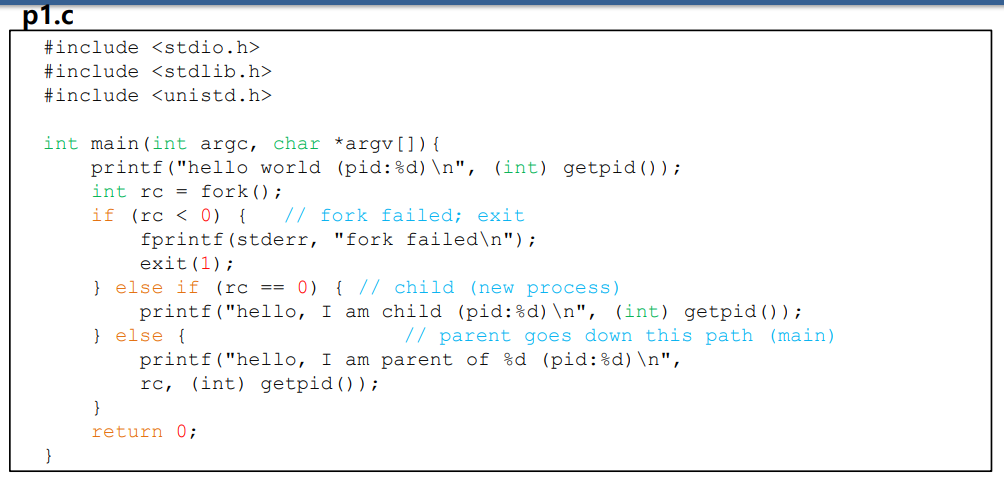
\includegraphics[width=17cm, height=8cm]{immagine_2025-01-23_124436468.png} % Percorso dell'immagine
   % \caption{Datagram Header} % Didascalia per l'immagine
    \label{fig:immagine} % Etichetta per riferimento
\end{figure}
\noindent
La \textbf{fork()} essendo una chiamata di sistema, è considerata un \textbf{servizio del kernel}. Ci consente di \textbf{sdoppiare} il processo che lo chiama, va a creare un nuovo processo che sarà un figlio del processo chiamante. La \textbf{fork} ritorna 0 se l'esecuzione continua sul processo figlio, ritorna \textbf{il pid del processo figlio} se l'esecuzione continua sul processo padre. Ritorna un valore \textbf{minore} di 0 se la fork fallisce.\\\\
\textbf{MAN}, fornisce una documentazione completa di qualsiasi chiamata di sistema. (es. man chiamataDiSistema)
\subsection{Chiamata di sistema: Wait()}
Attende il cambiamento di stato di un processo (a noi interessa la terminazione di un processo). 
\begin{figure}[H] % Usa 'H' per forzare la posizione qui
    \centering % Centra l'immagine
    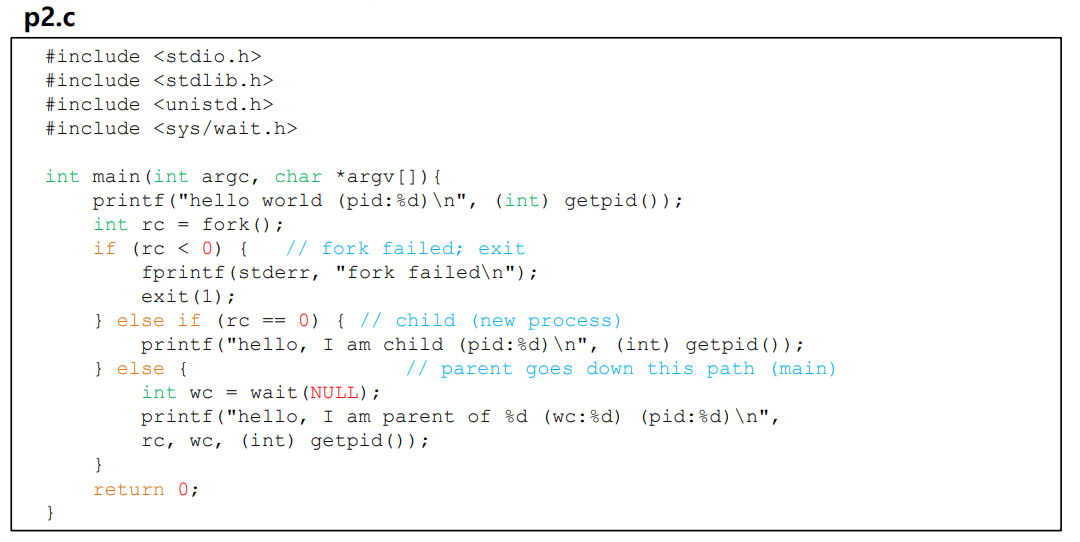
\includegraphics[width=17cm, height=8cm]{immagine_2025-01-23_130855260.png} % Percorso dell'immagine
   % \caption{Datagram Header} % Didascalia per l'immagine
    \label{fig:immagine} % Etichetta per riferimento
\end{figure}
\noindent
L'unica differenza con il programma di prima è quando l'esecuzione viene continuata dal processo padre. C'è una WAIT la quale ci aspetteremo che conterrà il valore del \textbf{processo che ha cambiato stato} (processo figlio). La vera \textbf{differenza} è che questa volta, il processo padre non potrà mai stampare la riga di testo se prima non muore il processo figlio (WAIT).\\\\
Se utilizziamo \textbf{WAIT PID} dobbiamo accertarci come processo padre di salvare da qualche parte tutti i processi figli che generiamo. Altra nota, le chiamate di sistema si trovano al capitolo 2 del MAN, quindi in caso ci fossero comandi con lo stesso nome della chiamata di sistema, dovremmo specificare il capitolo (man 2 write).
\subsection{Chiamata di sistema: Open(), Write(), Close()}
\textbf{Open()} ci serve per aprire un file, \textbf{Write()} ci serve per scrivere qualcosa all'interno di un file, \textbf{Close()} ci serve per chiudere il file precedentemente aperto.
 \begin{lstlisting}[language=C, frame=single, numbers=left]
#include <stdio.h>
#include <fcntl.h> // Da includere per utilizzare open
#include <string.h> //Da includere per utilizzare strlen
#include <unistd.h> //Da includere per utilizzare write

int main(){

    char messaggio[] = "Ciao!";
    int fd = open("pippo.txt", O_CREAT | O_TRUNC | O_WRONLY , S_IRWXU); 
    // fd sta per file descriptor
    write(fd, messaggio, strlen(messaggio));
    close(fd);
}
\end{lstlisting}
\noindent
\textbf{Importante}: Quando utilizziamo la open dobbiamo sempre specificare se vogliamo effettuare lettura (RDONLY), scrittura (WRONLY) o entrambe (RDWR). Il \textbf{file descriptor} è un numero intero ed è un riferimento al file che è stato aperto, infatti tutte le interazioni future verranno fatte utilizzando il riferimento del file descriptor. 
\subsubsection{Write()}
Quello che fa la \textbf{write} è prendere un puntatore all'inizio della memoria di messaggio (\textbf{secondo parametro} indirizzo di base della memoria dal quale devo iniziare a leggere i dati da scrivere da li vado avanti per quanto indicato dal \textbf{terzo parametro}) e va avanti per la lunghezza specificata dal terzo parametro. La write \textbf{ritorna} il numero di byte che sono stati scritti dalla chiamata stessa.
\section{Sesta lezione: process API}
Continuiamo a vedere \textbf{read e write}. \textbf{S IRWXU} ci dice i permessi che ha il file sul file system. 
 \begin{lstlisting}[language=C, frame=single, numbers=left]
#include <stdio.h>
#include <fcntl.h> // Da includere per utilizzare open
#include <string.h> //Da includere per utilizzare strlen
#include <unistd.h> //Da includere per utilizzare write

int main(){

    char messaggio[] = "Ciao!";
    int buffer = 4;
    int fd = open("pippo.txt", O_CREAT | O_TRUNC | O_WRONLY , S_IRWXU); 
    // fd sta per file descriptor
    printf("fd: %d\n", fd);
    int bytes = write(fd, &buffer, sizeof(int)); //in questo modo nel file pippo
    // verranno messi 4 caratteri "spazzatura"
    printf("bytes: %d\n, bytes);
    close(fd);
}
\end{lstlisting}
\noindent
Ora ci occupiamo della lettura.
 \begin{lstlisting}[language=C, frame=single, numbers=left]
#include <stdio.h>
#include <fcntl.h> // Da includere per utilizzare open
#include <unistd.h> //Da includere per utilizzare read

int main(){

    int fd = open("pippo.txt", O_RDONLY , S_IRWXU); 
    int buffer = 0;
    read(fd, &buffer, sizeof(int));
    printf("Buffer: %d\n", buffer);
    close(fd);
}
\end{lstlisting}
\subsection{Chiamata di sistema: Exec()}
La chiamata di sistema \textbf{Exec()} ci permette di eseguire altre applicazioni da applicazioni che noi stiamo scrivendo (andandone a richiamare l'eseguibile).
 \begin{lstlisting}[language=C, frame=single, numbers=left]
#include <stdio.h>
#include <fcntl.h> // Da includere per utilizzare open
#include <unistd.h> //Da includere per utilizzare read
#include <string.h> //Da includere per strdup

int main(){

    int fd = open("pippo.txt", O_RDONLY , S_IRWXU); 
    int buffer = 0;
    read(fd, &buffer, sizeof(int));
    printf("Buffer: %d\n", buffer);
    close(fd);

    char *myarg[2]; //array di argomenti per la exec
                    // Percorso dell'eseguibile
                    // Argomenti da passare all eseguibile
                    // Null ultimo argomento
    myarg[0] = strdup("ls");
    myarg[1] = NULL;
    execvp(myarg[0], myarg);
    
}
\end{lstlisting}
\noindent
\textbf{Strdup} si prende una stringa come parametro, fa una malloc per questa stringa ci mette dentro il contenuto della memoria che ha appena allocato e restituisce il puntatore a quell'area di memoria. Per quest'esempio utilizziamo \textbf{execvp}, la \textbf{famiglia v} mi permette di passare come parametri l'eseguibile nel formato array di stringhe, la \textbf{famiglia p} fa una ricerca all'interno della variabile d'ambiente path dell'eseguibile che voglio eseguire esattamente come se fossi all'interno della shell. Tutto ciò che c'è \textbf{sotto la exec} non verrà eseguito per questo motivo prima della exec si chiama una fork che chiamerà un altro processo a eseguire altri comandi.
\section{Settima lezione: introduzione programmazione concorrente}
Si va a svelare la soluzione del 4 esercizio della seconda esercitazione in laboratorio. (slide su my malloc).
\subsection{Testo dell'esercizio}
\begin{figure}[H] % Usa 'H' per forzare la posizione qui
    \centering % Centra l'immagine
    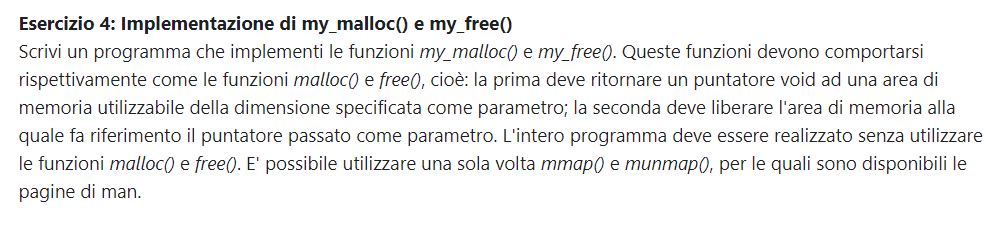
\includegraphics[width=17cm, height=4cm]{immagine_2025-01-23_153111376.png} % Percorso dell'immagine
   % \caption{Datagram Header} % Didascalia per l'immagine
    \label{fig:immagine} % Etichetta per riferimento
\end{figure}
\noindent
Quindi la funzione my malloc, dovrà prendere un argomento (dimensione) e ritornare un void$\ast$. La my free quindi dovrà prendere soltanto un puntatoree tornare un intero che ci faccia capire se è andata a buon fine o meno.
\\\\
\textbf{MMAP} è una funzione che possiamo utilizzare in due modi diversi: il \textbf{primo} modo è quello di simulare il comportamento della malloc (infatti prende più argomenti che in realtà la malloc mette di default es. permessi di memoria all area di memoria). Il \textbf{secondo} è quello di creare una mappa con nome: un riferimento in memoria rispetto a un file che si trova nel file system. Potremmo avere anche mappe anonime (quello che corrisponde a una malloc) le quali sono porzioni di memoria che non hanno un corrispettivo file nel file system. Il \textbf{primo} parametro della mmap è un'indirizzo di memoria che noi vorremmo come base di partenza per la memoria che vogliamo allocare (si può non specificare). \textbf{Secondo} parametro dimensione dell'area di memoria che vogliamo allocare. \textbf{Prot} indica i permessi. \textbf{Flags} lo utilizziamo per map shared e map private. Il \textbf{quinto} parametro è un fd e per finire abbiamo un offset ( che serve a dire da dove partire ).
\subsection{Idea della risoluzione}
Torniamo alla risoluzione dell'esercizio, l'idea è: uso mmap una volta per andare a fare l'allocazione di memoria, quest'area sarà tutta e sola l'area di memoria che il nostro computer andrà a utilizzare, infatti tutte le successive allocazioni con l'utilizzo della my malloc verranno erogate a partire da questa area di memoria che ho inizializzato con la mmap. Ho bisogno di scrivere da qualche parte quanto sto allocando in modo tale che la my free sappia quanto deve disallocare. A tal proposito uso una struttura dati che chiamo \textbf{Block$\ast$} che mi va a contenere una dimensione, se il blocco di memoria è libero e qual'è il prossimo blocco di memoria.
\\
Es. se volessi fare una my malloc di 1000 potrei farlo se decido di allocare ad esempio (1008 byte) ma mi rimarrebbero solo 8 byte per contenere i metadati con le informazioni sui blocchi di memoria.
\begin{figure}[H] % Usa 'H' per forzare la posizione qui
    \centering % Centra l'immagine
    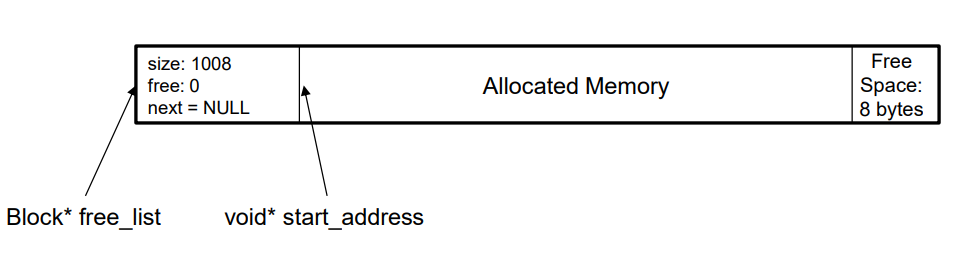
\includegraphics[width=17cm, height=4cm]{immagine_2025-01-23_160223158.png} % Percorso dell'immagine
   % \caption{Datagram Header} % Didascalia per l'immagine
    \label{fig:immagine} % Etichetta per riferimento
\end{figure}
\noindent
La my free va indietro di 16 byte rispetto a start address legge il blocco e sa quanta memoria deve liberare. La libera semplicemente settando a 1 la variabile free. Vediamo ora una my malloc da 100 byte.
\begin{figure}[H] % Usa 'H' per forzare la posizione qui
    \centering % Centra l'immagine
    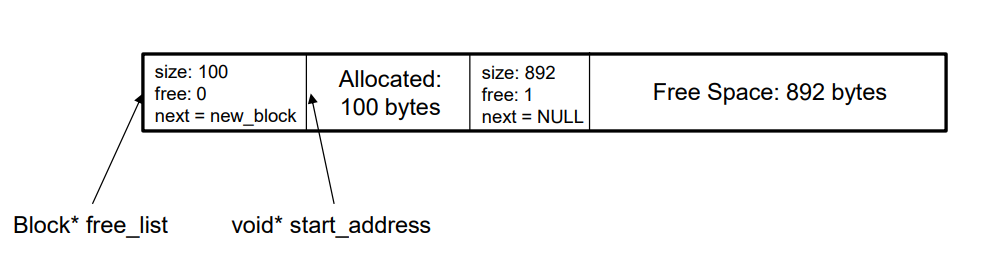
\includegraphics[width=17cm, height=4cm]{immagine_2025-01-23_160624295.png} % Percorso dell'immagine
   % \caption{Datagram Header} % Didascalia per l'immagine
    \label{fig:immagine} % Etichetta per riferimento
\end{figure}
\noindent
Quell' 892 è dato da $1024-16-100-16$. 
\begin{figure}[H] % Usa 'H' per forzare la posizione qui
    \centering % Centra l'immagine
    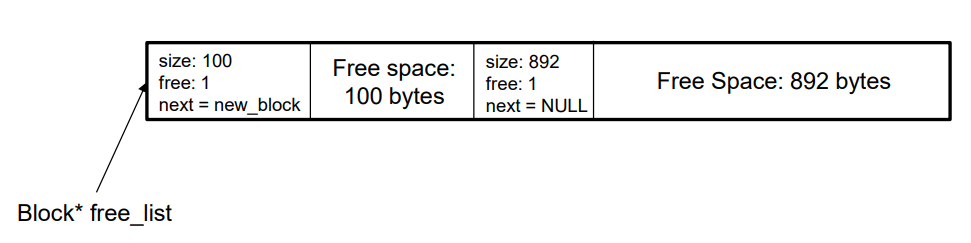
\includegraphics[width=17cm, height=4cm]{immagine_2025-01-23_161024907.png} % Percorso dell'immagine
   % \caption{Datagram Header} % Didascalia per l'immagine
    \label{fig:immagine} % Etichetta per riferimento
\end{figure}
\noindent
Ora posso liberare la memoria cambiando semplicemente il parametro free. Il problema è che la memoria non essendo contigua posso utilizzare semplicemente solamente 992 byte (problema della frammentazione interna). La soluzione è quella di fare un merge di blocchi liberi adiacenti.
\begin{figure}[H] % Usa 'H' per forzare la posizione qui
    \centering % Centra l'immagine
    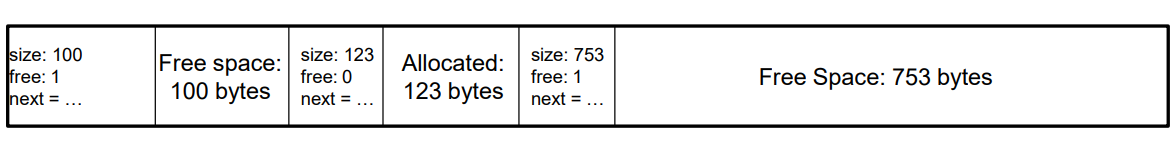
\includegraphics[width=18cm, height=3cm]{immagine_2025-01-23_161300735.png} % Percorso dell'immagine
   % \caption{Datagram Header} % Didascalia per l'immagine
    \label{fig:immagine} % Etichetta per riferimento
\end{figure}
\noindent
Se avessimo una situazione del genere, non potremmo risolverla.
\subsection{Soluzione in C}
Abbiamo due macro una per la dimensione della memoria che vogliamo utilizzare e una per definire la dimensione minima del blocco che posso creare. La struct del blocco è fatta esattamente come viene specificato nelle slide (size$\_$t size, int free e struct Block$\ast$ next). 
\subsubsection{init$\_$memory$\_$pool()}
\begin{figure}[H] % Usa 'H' per forzare la posizione qui
    \centering % Centra l'immagine
    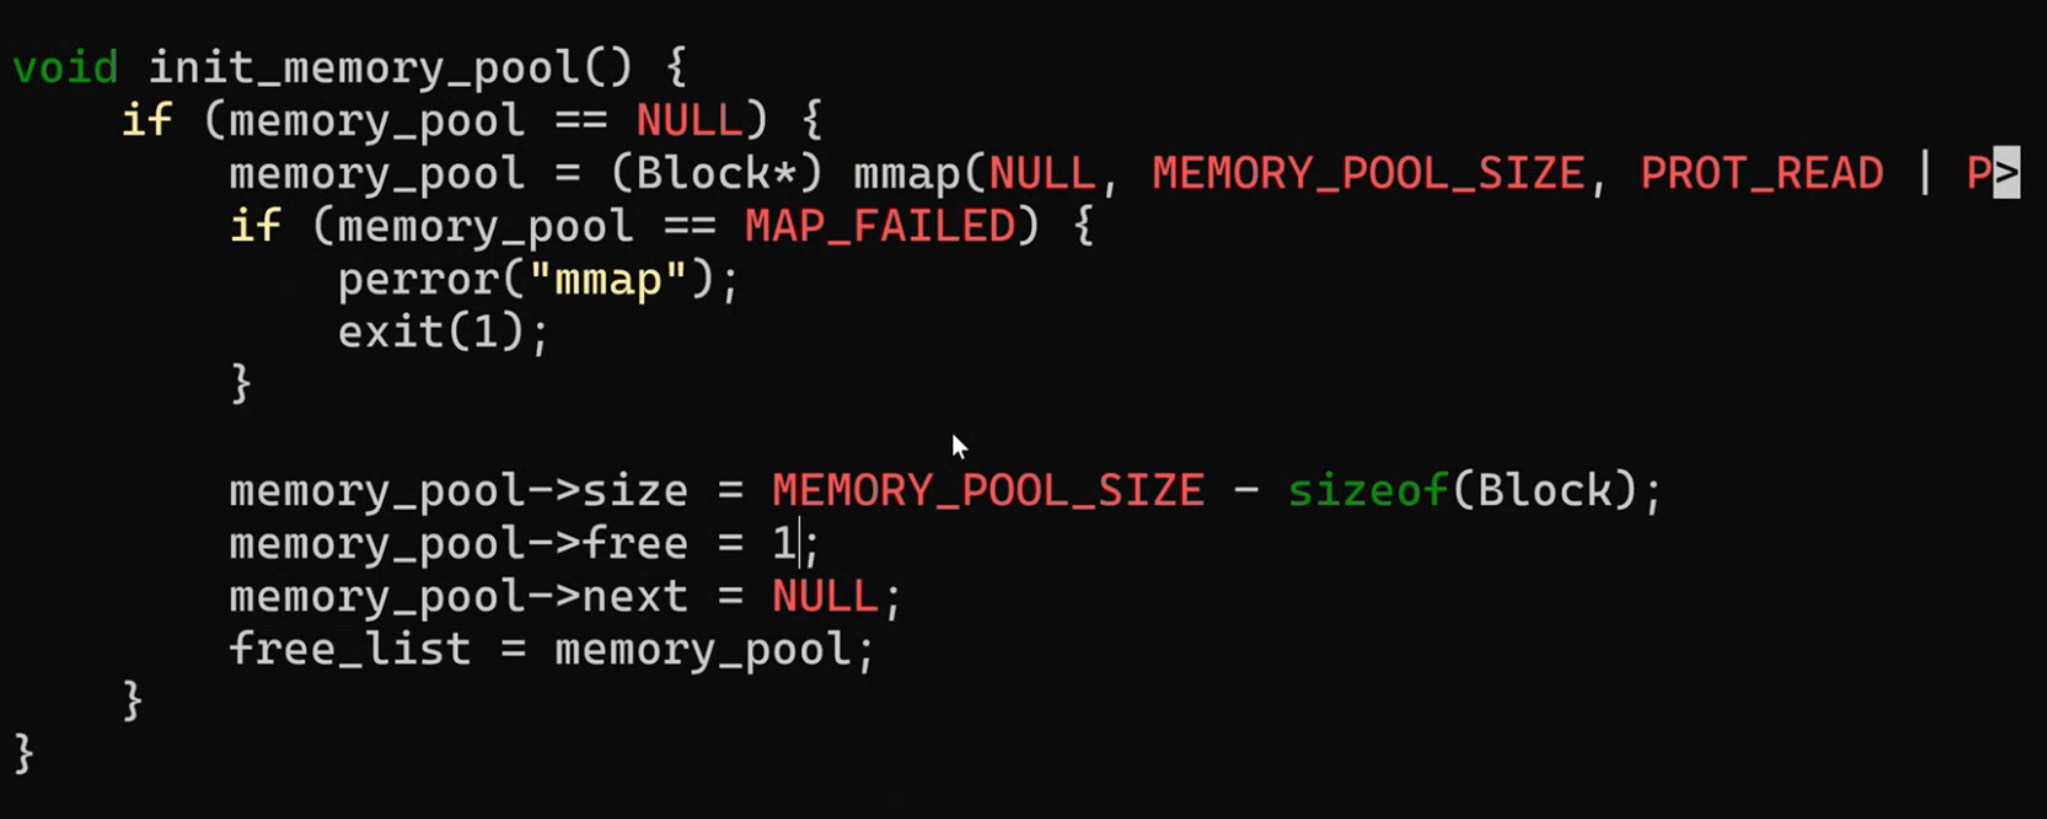
\includegraphics[width=18cm, height=5cm]{IMG_0843.jpeg} % Percorso dell'immagine
   % \caption{Datagram Header} % Didascalia per l'immagine
    \label{fig:immagine} % Etichetta per riferimento
\end{figure}
\noindent
Per prima cosa vado a inizializzare il \textbf{memory pool} (mettere il pezzettino di memoria all'inizio che mi dice la memoria utilizzabile). Se \textbf{memory pool} è nullo allora lo vado a creare con \textbf{mmap} (parametri: NULL(non ci interessa suggerire l'indirizzo da cui partire), memory pool size (dimensione che vogliamo allocare), i prot che inseriamo sono read e write dato che vogliamo leggerla e scriverla, dopodichè diciamo che la mappa deve essere privata e anonima essendo anonima fd=-1 e l offset non è specificato). Le istruzioni dopo sono in linea col funzionamento spiegato prima (imposto i parametri).
\subsubsection{split$\_$block}
\begin{figure}[H] % Usa 'H' per forzare la posizione qui
    \centering % Centra l'immagine
    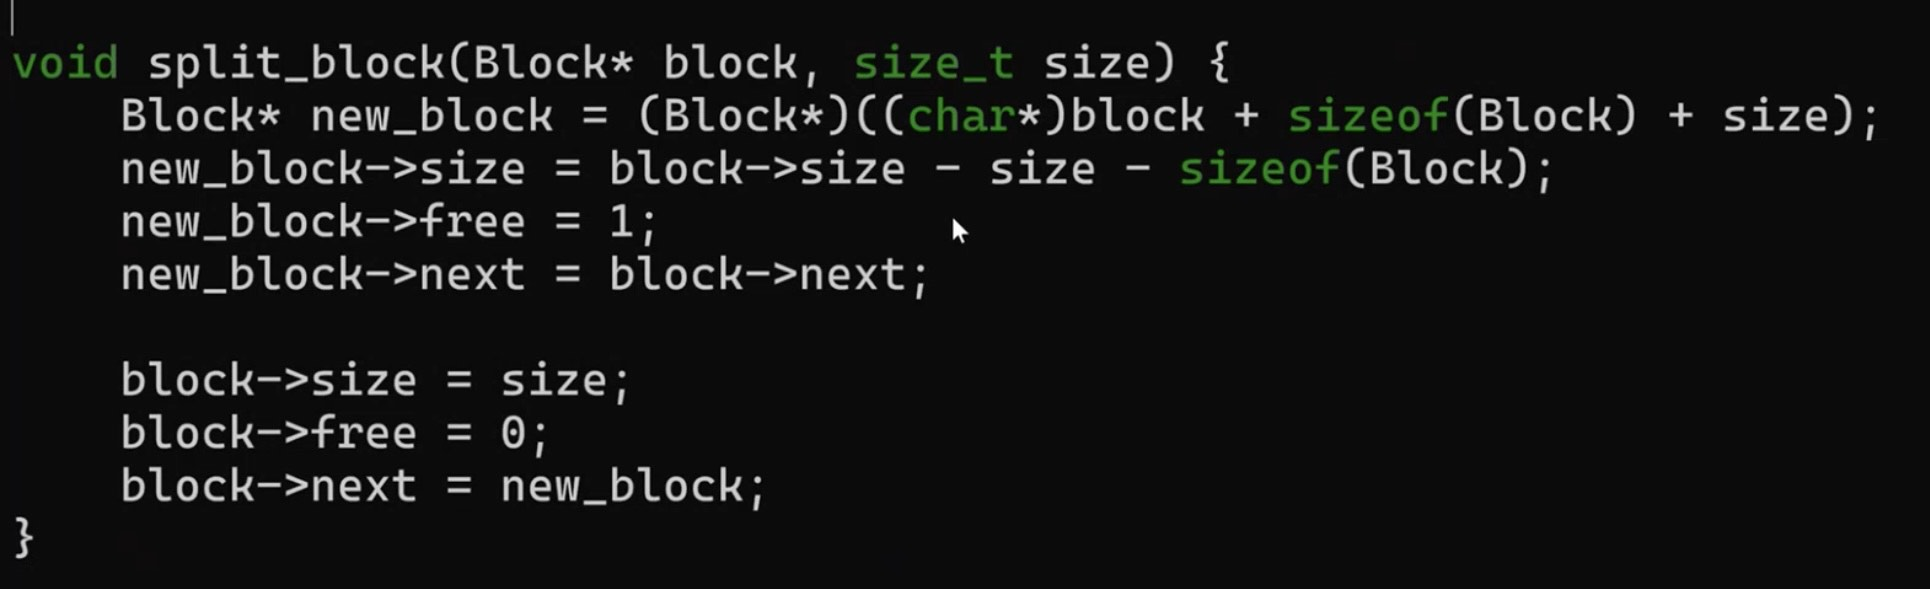
\includegraphics[width=18cm, height=4cm]{IMG_0844.jpeg} % Percorso dell'immagine
   % \caption{Datagram Header} % Didascalia per l'immagine
    \label{fig:immagine} % Etichetta per riferimento
\end{figure}
\noindent
Richiesta di allocazione che permette successive richieste di allocazione. Creo un puntatore di base al nuovo blocco creato a partire da: il blocco corrente (quello che voglio splittare) + dimensione della struttura dati del blocco + dimensione dei dati allocati per quel blocco. La dimensione del nuovo blocco che andiamo a creare è quindi la dimensione del blocco che ho a disposizione - la dimensione dei dati che stiamo andando a utilizzare - dimensione del blocco che ho creato.
\subsubsection{print$\_$blocks}
\begin{figure}[H] % Usa 'H' per forzare la posizione qui
    \centering % Centra l'immagine
    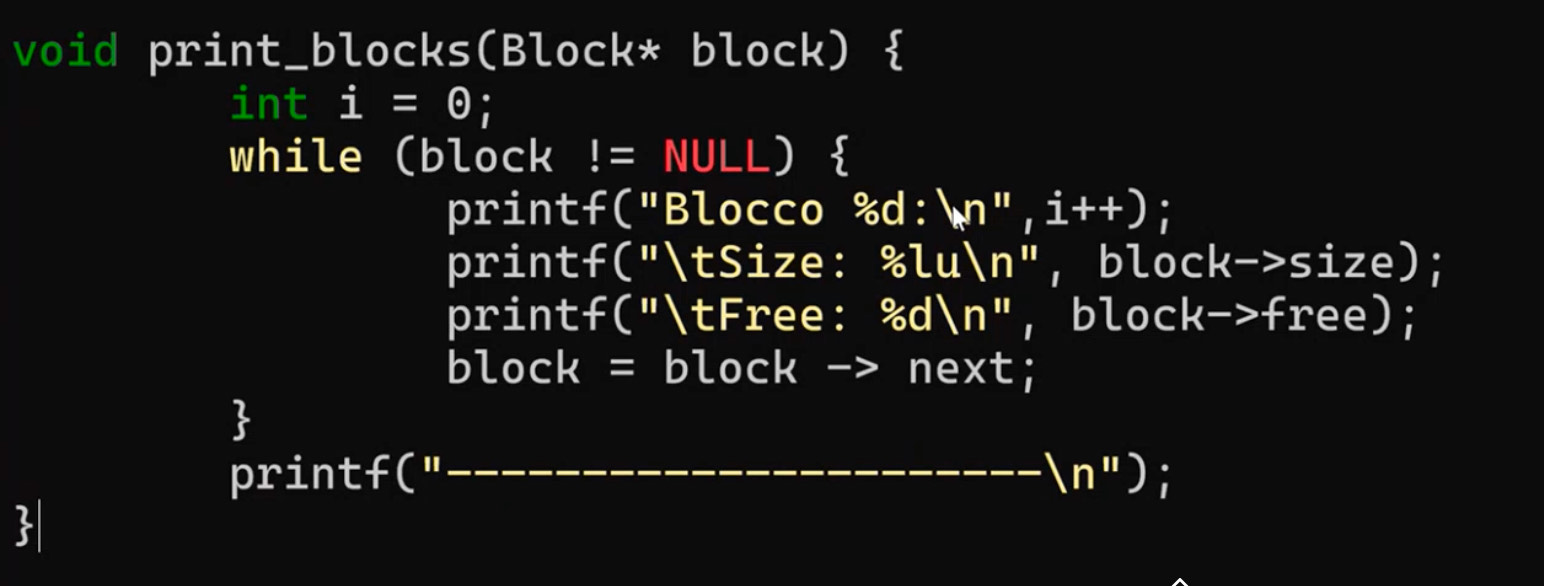
\includegraphics[width=18cm, height=4cm]{IMG_0845.jpeg} % Percorso dell'immagine
   % \caption{Datagram Header} % Didascalia per l'immagine
    \label{fig:immagine} % Etichetta per riferimento
\end{figure}
\noindent
\subsubsection{my$\_$malloc}
\begin{figure}[H] % Usa 'H' per forzare la posizione qui
    \centering % Centra l'immagine
    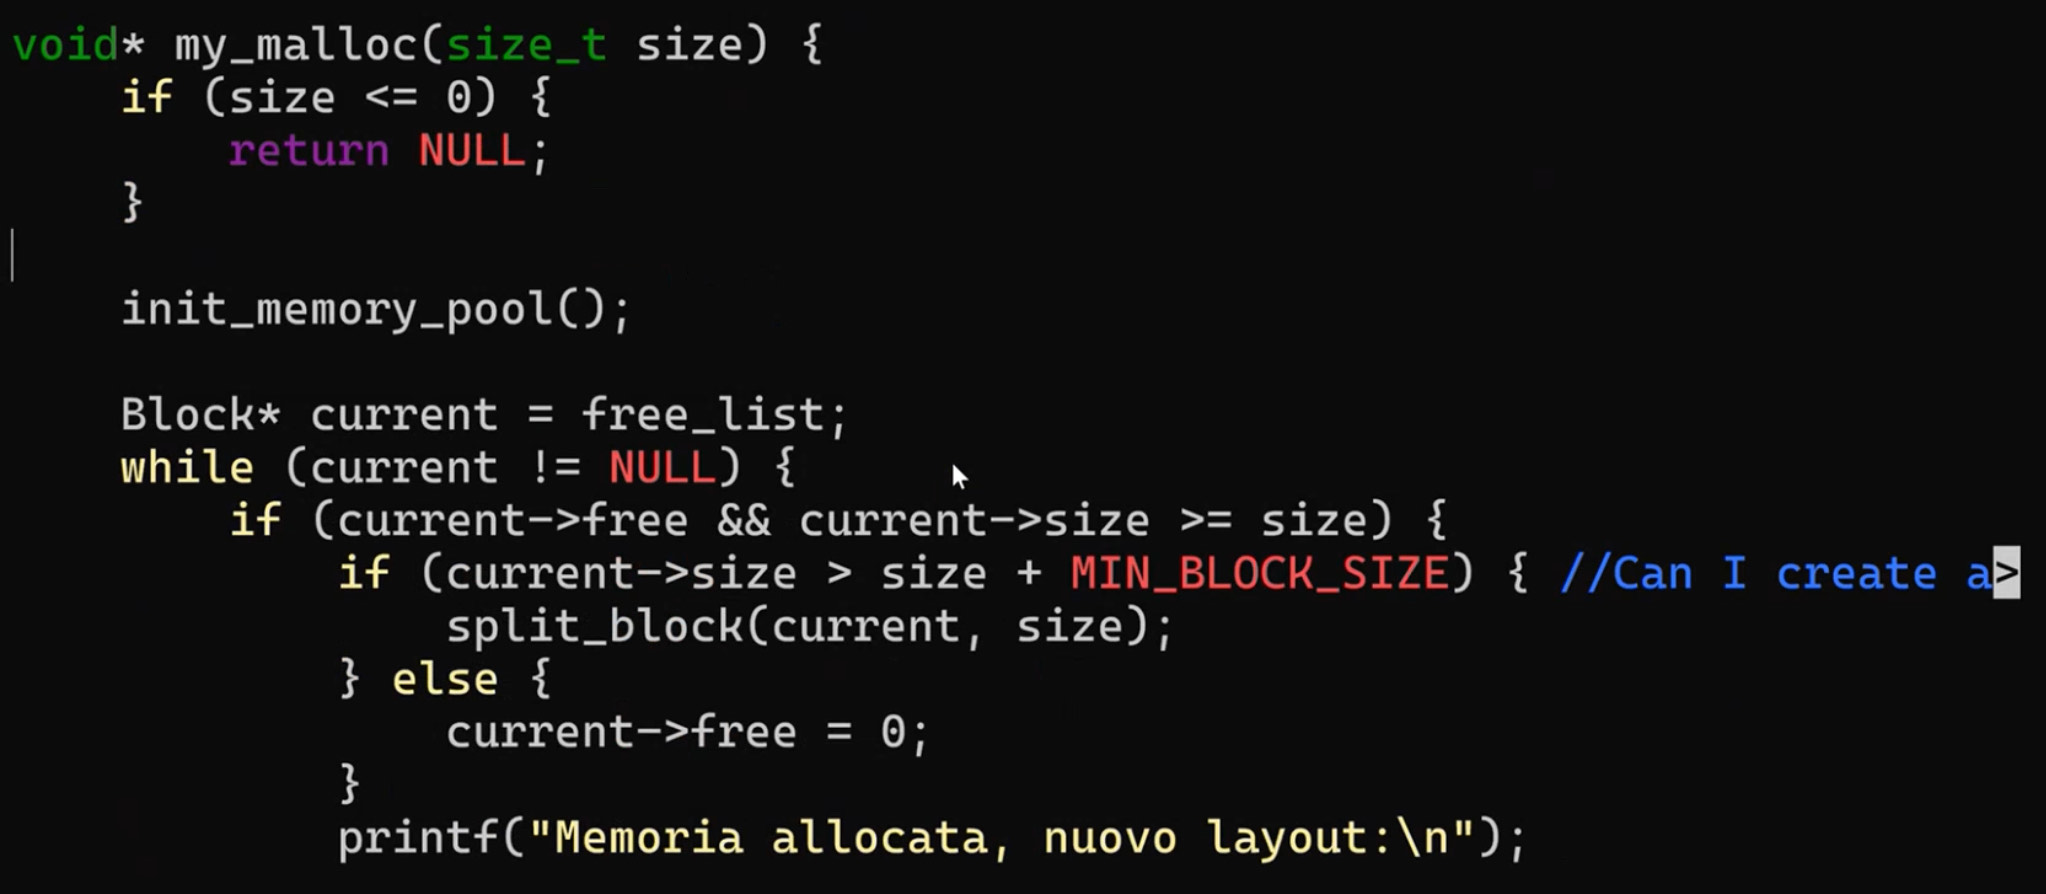
\includegraphics[width=18cm, height=5cm]{IMG_0846.jpeg} % Percorso dell'immagine
   % \caption{Datagram Header} % Didascalia per l'immagine
    \label{fig:immagine} % Etichetta per riferimento
\end{figure}
\noindent
Quindi la nostra my malloc ritorna e prende i parametri precedentemente citati, quindi sostanzialmente partiamo dall'inizio dei blocchi fino a quando non troviamo un blocco di dimensione sufficiente alla richiesta che è stata fatta. Quindi se entra un'altro blocco andiamo a richiamare split block sennò dichiariamo tutta la memoria restante occupata. Andiamo quindi a ritornare l'indirizzo di base della memoria allocata.
\begin{figure}[H] % Usa 'H' per forzare la posizione qui
    \centering % Centra l'immagine
    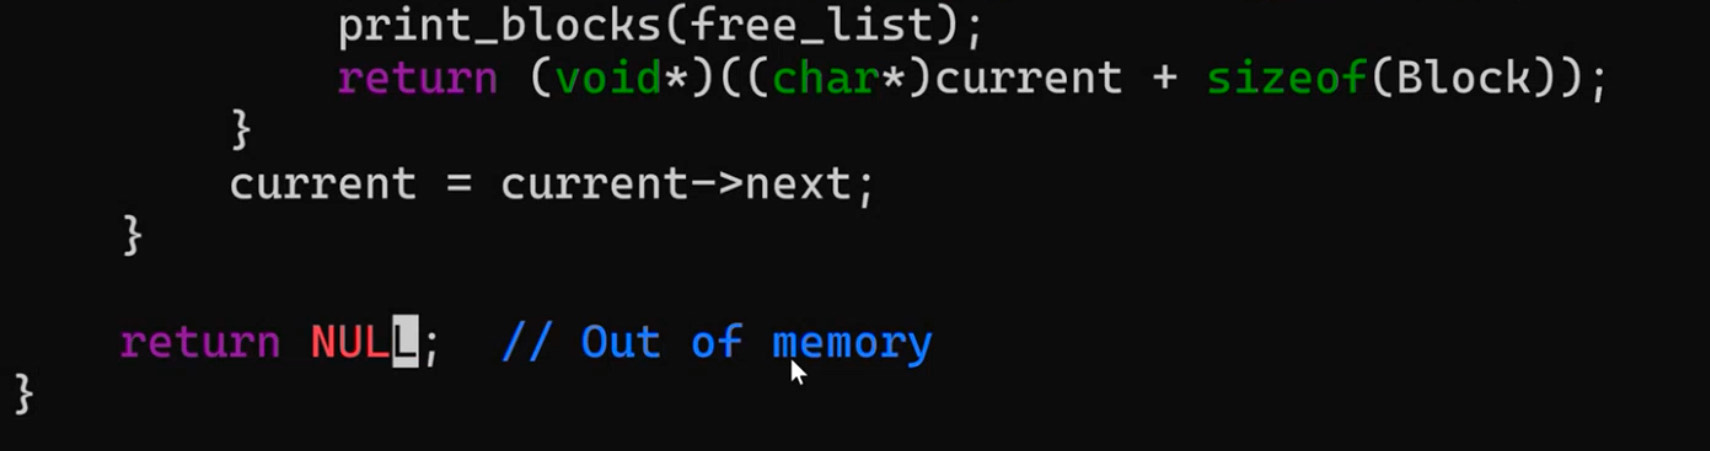
\includegraphics[width=18cm, height=3cm]{IMG_0848.jpeg} % Percorso dell'immagine
   % \caption{Datagram Header} % Didascalia per l'immagine
    \label{fig:immagine} % Etichetta per riferimento
\end{figure}
\noindent
\subsubsection{merge$\_$blocks}
\begin{figure}[H] % Usa 'H' per forzare la posizione qui
    \centering % Centra l'immagine
    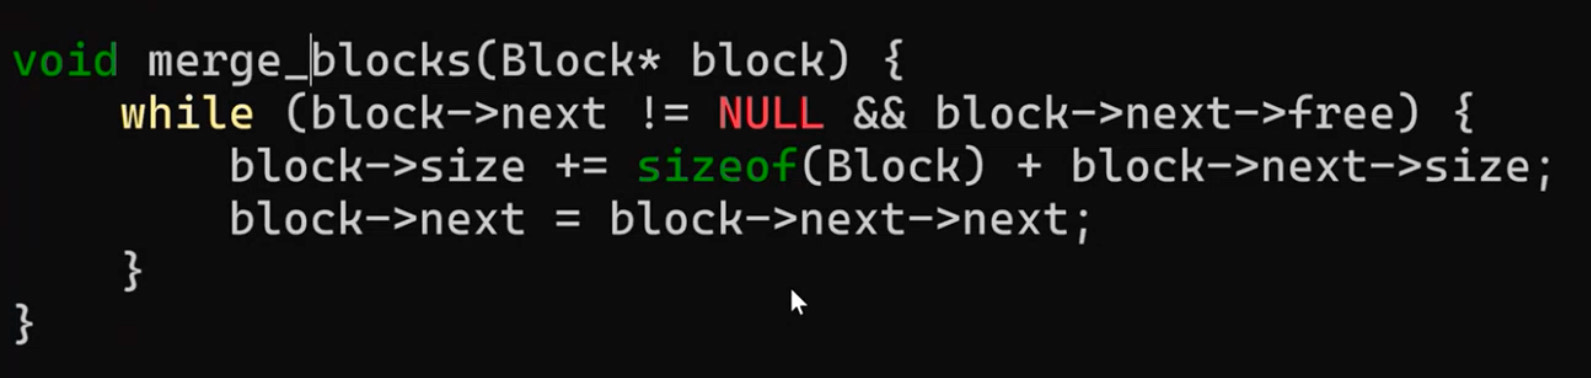
\includegraphics[width=18cm, height=3cm]{IMG_0849.jpeg} % Percorso dell'immagine
   % \caption{Datagram Header} % Didascalia per l'immagine
    \label{fig:immagine} % Etichetta per riferimento
\end{figure}
\noindent
\subsubsection{my$\_$free}
\begin{figure}[H] % Usa 'H' per forzare la posizione qui
    \centering % Centra l'immagine
    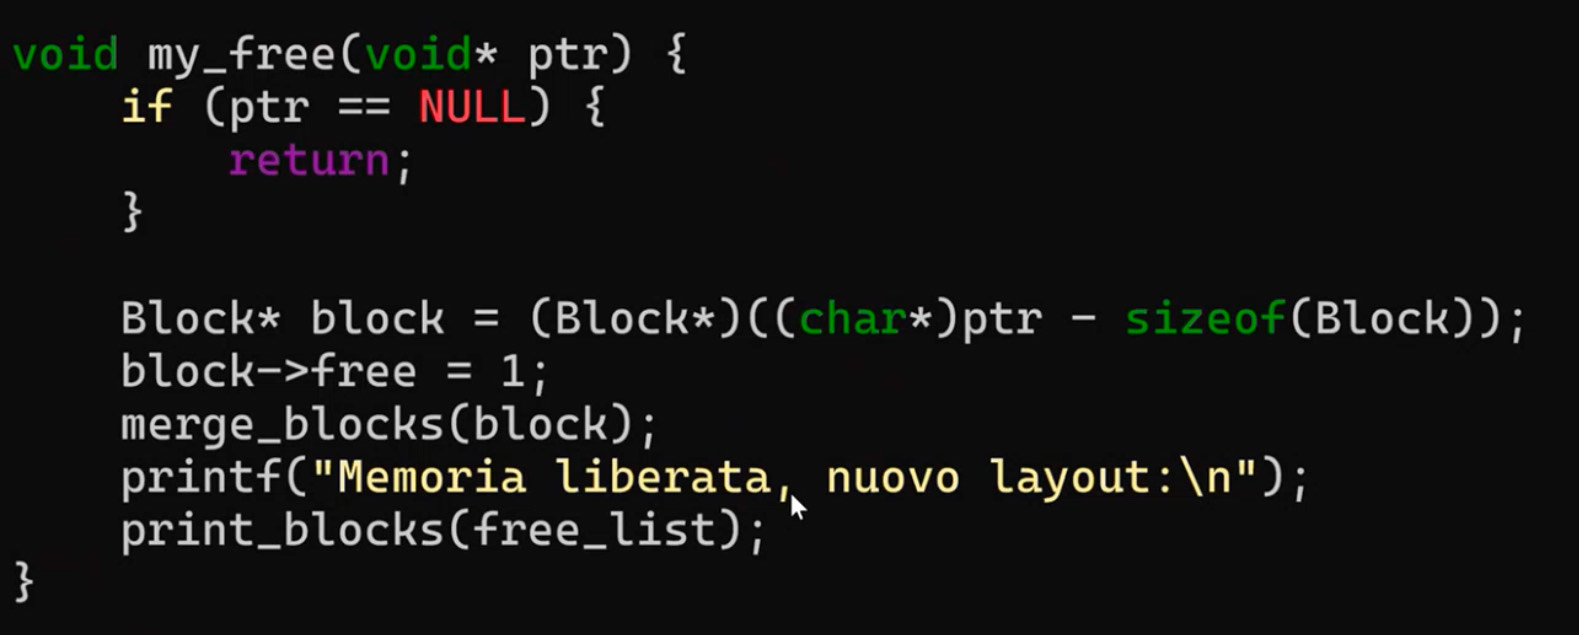
\includegraphics[width=18cm, height=4cm]{IMG_0850.jpeg} % Percorso dell'immagine
   % \caption{Datagram Header} % Didascalia per l'immagine
    \label{fig:immagine} % Etichetta per riferimento
\end{figure}
\noindent
Prendo il puntatore passato e ci sottraggo la dimensione dei metadati in modo tale da liberare la memoria.
\subsubsection{cleanup$\_$memory$\_$pull}
\begin{figure}[H] % Usa 'H' per forzare la posizione qui
    \centering % Centra l'immagine
    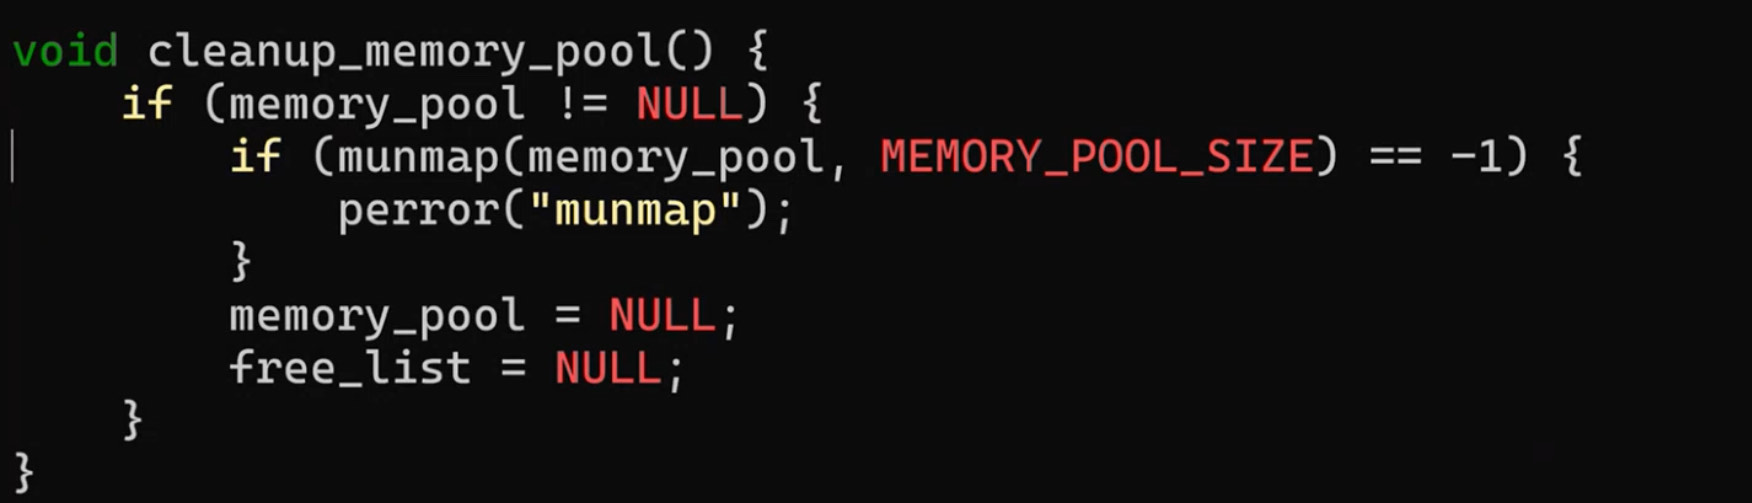
\includegraphics[width=18cm, height=3cm]{IMG_0852.jpeg} % Percorso dell'immagine
   % \caption{Datagram Header} % Didascalia per l'immagine
    \label{fig:immagine} % Etichetta per riferimento
\end{figure}
\noindent
\subsubsection{Main}
\begin{figure}[H] % Usa 'H' per forzare la posizione qui
    \centering % Centra l'immagine
    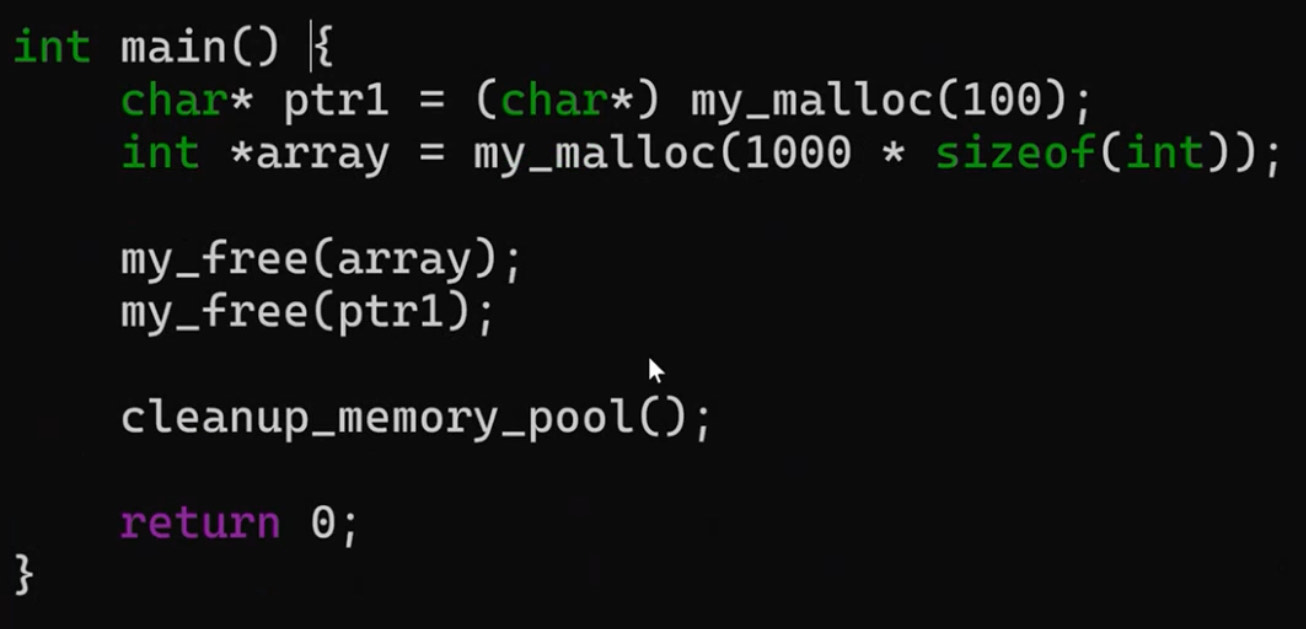
\includegraphics[width=18cm, height=4cm]{IMG_0851.jpeg} % Percorso dell'immagine
   % \caption{Datagram Header} % Didascalia per l'immagine
    \label{fig:immagine} % Etichetta per riferimento
\end{figure}
\noindent
\subsection{Programmazione Concorrente}
Gestione degli interrupt. Ogni processo ha un \textbf{pc (program counter)}. In applicazioni multi thread si possono avere più \textbf{program counter}. Una differenza sostanziale è che tutti i thread si appoggiano allo stesso spazio degli indirizzi, cosa non possibile nella programmazione multi processo. Ogni thread ha quindi il proprio insieme di \textbf{registri}. Con i thread si fa un context switch più leggero e i loro dati vengono salvati in memoria in un \textbf{Thread Control Blocks (TCBs)}. Come cambia lo spazio degli indirizzi:
\begin{figure}[H] % Usa 'H' per forzare la posizione qui
    \centering % Centra l'immagine
    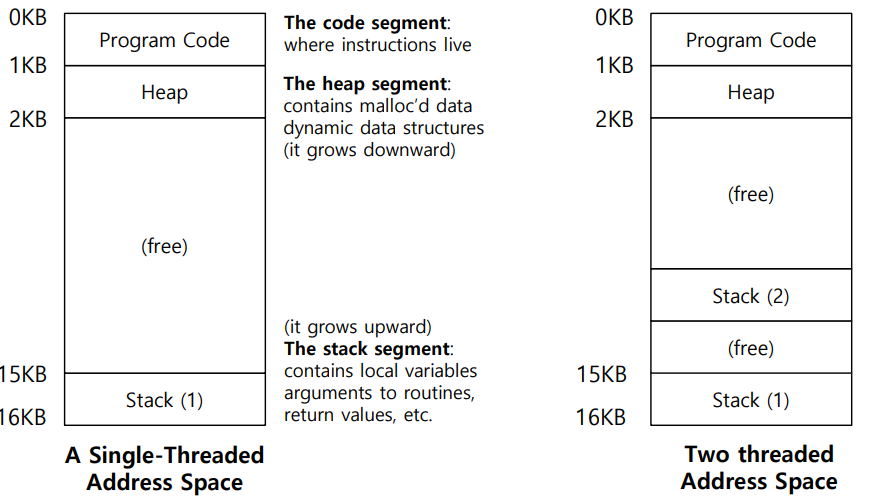
\includegraphics[width=15cm, height=5cm]{immagine_2025-01-23_174622346.png} % Percorso dell'immagine
   % \caption{Datagram Header} % Didascalia per l'immagine
    \label{fig:immagine} % Etichetta per riferimento
\end{figure}
\noindent
La programmazione multi thread va a migliorare l'efficienza.
\subsubsection{Primo esempio sulla programmazione multi thread}
\begin{figure}[H] % Usa 'H' per forzare la posizione qui
    \centering % Centra l'immagine
    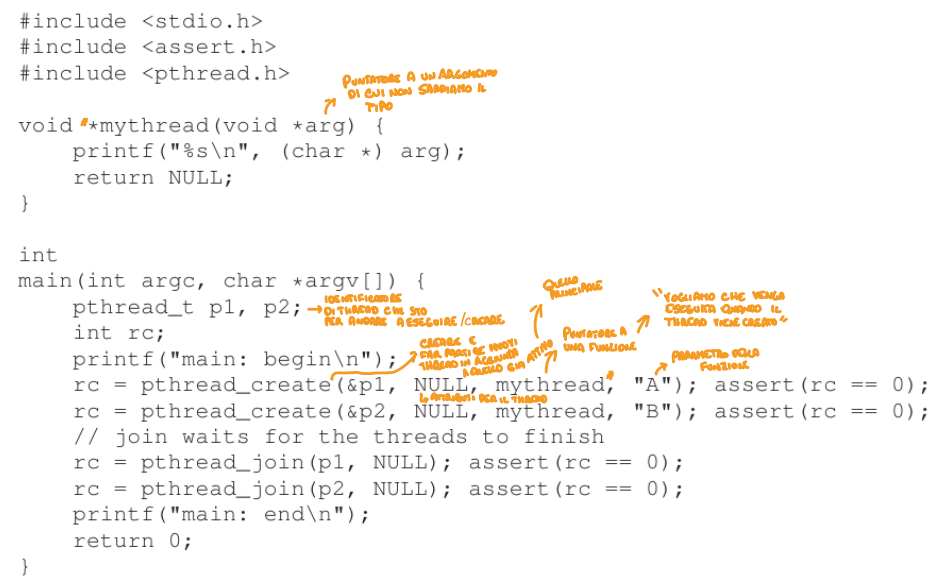
\includegraphics[width=15cm, height=8cm]{immagine_2025-01-23_175022336.png} % Percorso dell'immagine
   % \caption{Datagram Header} % Didascalia per l'immagine
    \label{fig:immagine} % Etichetta per riferimento
\end{figure}
\noindent
Utilizzeremo applicazioni che fanno uso di \textbf{Pthread} (libreria più utilizzata per programmazione concorrente in c). Le prime due variabili di tipo \textbf{Pthread$\_$t} sono degli identificatori ai thread che sto per andare a creare/eseguire. Successivamente utilizziamo \textbf{pthread$\_$create} è la funzione che fa si che un thread possa nascere e possa essere eseguito. Gli passiamo come \textbf{argomenti}: un riferimento a oggetto di tipo pthread$\_$t che può andare a modificare, il terzo argomento è un puntatore a una funzione, l'ultimo parametro è un argomento da passare alla funzione. Quindi quando questa funzione viene eseguita, quello che succede è che oltre al thread principale verranno creati due nuovi thread con i propri pc. \textbf{Pthread$\_$join} il thread che va a eseguire quella funzione si mette in attesa del thread identificativo p1 (il thread principale non andrà avanti fino a che p1 non avrà terminato la sua esecuzione).
\subsubsection{Possibili scenari di esecuzione}
\begin{figure}[H]
    \begin{minipage}[b]{0.45\textwidth} % Prima figura a sinistra
        \centering
        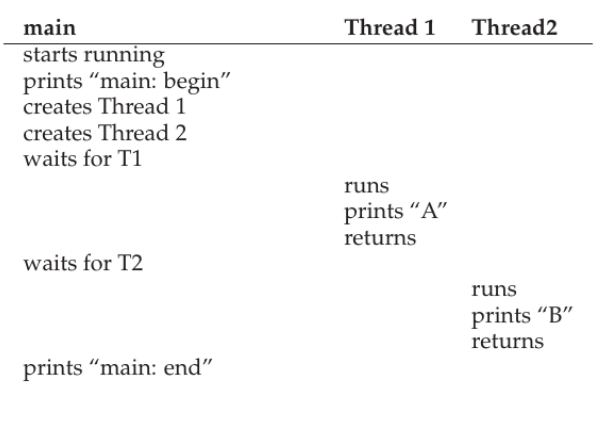
\includegraphics[width=8cm, height=4cm]{Screenshot 2025-01-23 180248.png} % Sostituisci con il nome del tuo file immagine
       % \caption{Tree Search}
    \end{minipage}
    \hfill
    \begin{minipage}[b]{0.45\textwidth} % Seconda figura a destra
        \centering
        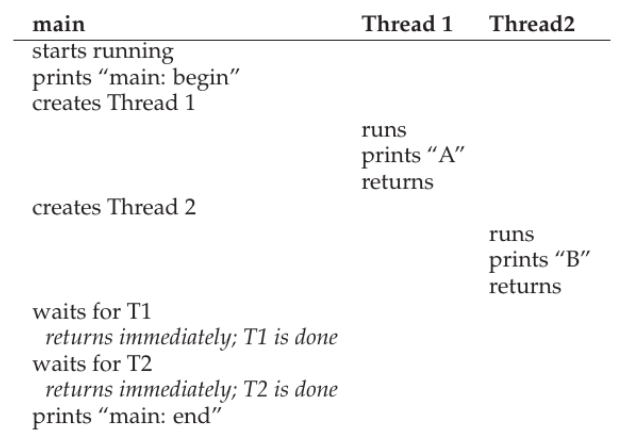
\includegraphics[width=8cm, height=4cm]{Screenshot 2025-01-23 180257.png} % Sostituisci con il nome del tuo file immagine
       % \caption{Graph Search}
    \end{minipage}
\end{figure}
\begin{figure}[H] % Usa 'H' per forzare la posizione qui
    \centering % Centra l'immagine
    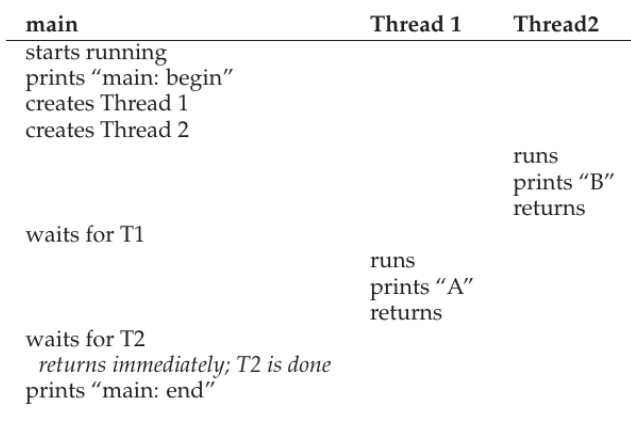
\includegraphics[width=8cm, height=4cm]{Screenshot 2025-01-23 180307.png} % Percorso dell'immagine
   % \caption{Datagram Header} % Didascalia per l'immagine
    \label{fig:immagine} % Etichetta per riferimento
\end{figure}
\noindent
Esecuzioni che dipendono dallo scheduler. Il codice è nel container se vuoi eseguirlo devi togliere le include "" e mettere le p minuscole alle funzioni. Se voglio compilare qualcosa che fa uso di \textbf{pthread} devo scrivere \textbf{gcc -o t0 t0.c -pthread}
\subsubsection{Pthread$\_$create}
\begin{figure}[H] % Usa 'H' per forzare la posizione qui
    \centering % Centra l'immagine
    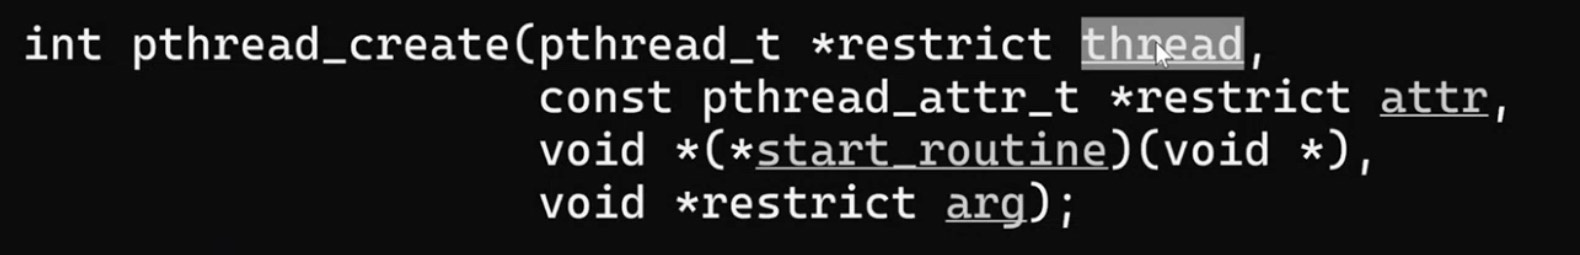
\includegraphics[width=12cm, height=3cm]{IMG_0853.jpeg} % Percorso dell'immagine
   % \caption{Datagram Header} % Didascalia per l'immagine
    \label{fig:immagine} % Etichetta per riferimento
\end{figure}
\noindent
Il primo argomento è un puntatore a pthread t che sarà l'identificatore del thread che abbiamo creato. Poi c'è la variabile che definisce gli attributi specifici del thread che stiamo andando a creare. Il terzo parametro è il puntatore a funzione (indirizzo di memoria dove inizia quella funzione (quello che verrà messo dentro il pc del thread che stiamo andano a creare)). L'ultimo sono gli argomenti da passare al thread.
\subsubsection{Pthread$\_$join}
\begin{figure}[H] % Usa 'H' per forzare la posizione qui
    \centering % Centra l'immagine
    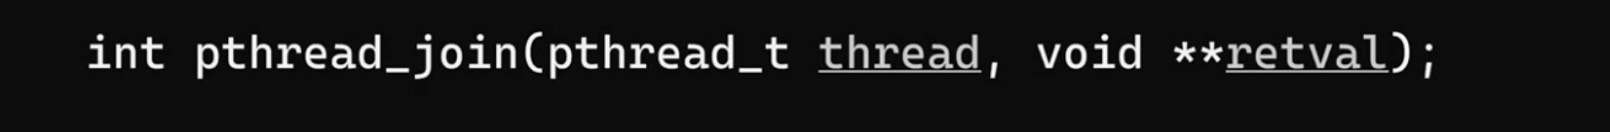
\includegraphics[width=14cm, height=2cm]{IMG_0854.jpeg} % Percorso dell'immagine
   % \caption{Datagram Header} % Didascalia per l'immagine
    \label{fig:immagine} % Etichetta per riferimento
\end{figure}
\noindent
Il secondo parametro è un doppio puntatore a un valore tornato dal thread.
\section{Ottava lezione: continuo su programmazione concorrente}
Inizialmente ci mostra come migliora l'esecuzione sfruttando la programmazione concorrente. 
\subsection{Moltiplicazione tra matrici (senza thread)}
Ci fa vedere le statistiche sui tempi di esecuzione con la funzione \textbf{gettimeofday}, non utilizziamo una semplice time perchè lavora a una grana troppo grossa e vogliamo qualcosa di più \textbf{preciso}. Questa funzione si appoggia a una struct di tipo \textbf{timeval}: una struttura composta di due campi uno per i secondi e uno per i microsecondi. Come primo parametro prende un riferimento a variabili di tipo \textbf{timeval} (es. start) in modo tale che prenda secondi e microsecondi.
\subsection{Moltiplicazione tra matrici (con thread)}
Ogni thread lavorerà su un sott'insieme di righe della matrice, l'esecuzione è migliore. Ci fa vedere poi il file che si trova nella home \textbf{.wslconfig}. Se lo apro vedo il numero di processori impostati, per cambiarli, li cambio sul file, stoppo il container, digito \textbf{wsl --shutdown} che va a riavviare la macchina virtuale sottostante ai container, applicando l'impostazione.
\subsection{Produttore-Consumatore}
Quest'esercizio riprende un tipo di \textbf{architettura software} su cui molto spesso ci si va a lavorare. Funzione con almeno due agenti uno che \textbf{produce} qualche tipo di informazione, uno che \textbf{consuma} l'informazione. I due condividono una struttura dati per comunicare, il produttore mette all'interno di una \textbf{pila} l'informazione, il consumatore la preleva e ci lavora sopra. Questo problema è di \textbf{sincronizzazione} tra i due thread (agenti). Ci suggerisce l'utilizzo di random e usleep (diversifica da sleep perchè ci fa attendere micro secondi la u sta per $\mu$).
 \begin{lstlisting}[language=C, frame=single, numbers=left]
#include <stdio.h>
#include <stdlib.h> // per la calloc e la random
#include <unistd.h> // per la usleep
#include <pthread.h> // per i thread

#define SIZE 10

struct stack{

    int* array;
    int capacita;
    int occupati;
    
}stack;

stack pila;

pthread_mutex_t lock = PTHREAD_MUTEX_INITIALIZER; // per sincronizzare i thread

void init(){

    pila.array = (int*) calloc(SIZE, sizeof(int));
    pila.capacita=SIZE;
    pila.occupati=0;
    
}

void push(int v){

    if (pila.occupati < pila.capacita){

        pila.array[pila.occupati] = v;
        pila.occupati++;
    }
}

//int perche vogliamo che ci restituisca l'ultimo elemento che era stato inserito
int pop(){

    int ret=-1;
    if (pila.occupati > 0){

        ret = pila.array[pila.occupati-1];
        pila.occupati--;
    }

    return ret;
}

void* produttore(void* arg){

    while (1){

        // Attesa random
        usleep(random()%1e6);
        pthread_mutex_lock(&lock);
        // Controllo se la pila e libera
        if( pila.occupati < pila.capacita ){
            // Elementi da inserire nella pila
            int elementi = random() % (pila.capacita - pila.occupati);
            for (int i = 0; i< elementi; i++){

                int v = random();
                push(random());
                printf("[Produttore] Inserito %d\n", v); 
            }
    }
    pthread_mutex_unlock(&lock);
}

}

void* consumatore(void* arg){

    while (1){

        usleep(random()%(int)1e6);
        pthread_mutex_lock(&lock);
        if (pila.occupati > 0){

            int elementi = random() % pila.occupati;
            for ( int i=0; i < elementi ; i++ ){

                int v = pop();
                printf("[Consumatore] Letto %d\n", v); 
            }
        }
        pthread_mutex_unlock(&lock);
    }
}


int main(){

    init();
    pthread_t prod, cons;

    pthread_create(&prod, NULL, produttore, NULL);
    pthread_create(&cons, NULL, consumatore, NULL);

    pthread_join(prod, NULL);
    pthread_join(cons, NULL);
}
\end{lstlisting}
\noindent
Per prima cosa creo la \textbf{struttura dati} con cui voglio lavorare. Creo una funzione che mi permetta di inizializzare la struttura dati. Quello che inizia con define è una macro. Ora creo \textbf{push} e \textbf{pop}. Dopo aver implementato tutto quello che serve per la struttura dati vado a implementare le funzioni \textbf{produttore} e \textbf{consumatore}. Random e 1e6 ($10^6$) sono di due tipi diversi, random è considerato un long int 1e6 un double, quindi bisogna fare un \textbf{cast} su 1e6. Una volta implementati gli elementi da inserire nella pila, ci ricordiamo che dobbiamo attendere il consumatore. Infatti se lo spazio è pieno, devo soltanto attendere fino a che non mi si libera dello spazio. Nel consumatore, posso andare a \textbf{prelevare} soltanto se c'è qualcosa nella pila. Il \textbf{problema} sta nel fatto che dobbiamo sincronizzare la pila su cui avvengono push e pop e la variabile pila occupati. Il professore continua a consigliare fortemente l'utilizzo del man. Se lasciassimo l'implementazione con solamente pthread create il \textbf{thread principale} finirebbe prima degli altri due e quindi l esecuzione terminerebbe. A tal proposito utilizziamo \textbf{pthread join} che fa si che il thread principale aspetti l'esecuzione dei figli. A questo punto il programma non sarebbe del tutto corretto, vi sono da verificare le \textbf{race condition}. Infatti il programma sembra funzionare a causa del fatto che l'attesa fa si che i thread non si sovrappongano ma in realtà potremmo sfociare in \textbf{segmentation fault}. Quindi se il \textbf{produttore} sta inserendo qualcosa all'interno della pila, il \textbf{consumatore} deve aspettare, se il \textbf{consumatore} sta rimuovendo dalla pila, il \textbf{produttore} deve aspettare. A tal proposito utilizzo \textbf{pthread mutex lock} e \textbf{unlock}.
\section{Richiamo teorico sui Lock}
\subsection{Sezione critica e Race Condition}
\textbf{Sezione critica}: è un pezzo di codice che è potenzialmente eseguito da più thread, che accedono a una variabile condivisa nello stesso momento. Più thread che eseguono una sezione critica possono risultare in\\
\textbf{Race condition}: il risultato della computazione dipende dal tempo di esecuzione del codice.\\
Per risolvere questo problema, abbiamo bisogno di un meccanismo flessibile, un meccanismo permetta di accedere a un thread alla volta alla sezione critica
\subsection{Lock}
Un \textbf{lock} è una variabile che contiene informazioni su quale thread può eseguire la sezione critica. L'idea di base è: la variabile lock mantiene lo stato del lock che può essere \textbf{disponibile} (nessun thread tiene il lock) o \textbf{acquisito} (un thread ha il lock e presumibilmente è nella sezione critica). \textbf{Mutex} (Mutua Escluzione) è il nome che la libreria POSIX usa per un lock. Viene utilizzata per la \textbf{mutua esclusione} tra thread.
\begin{figure}[H] % Usa 'H' per forzare la posizione qui
    \centering % Centra l'immagine
    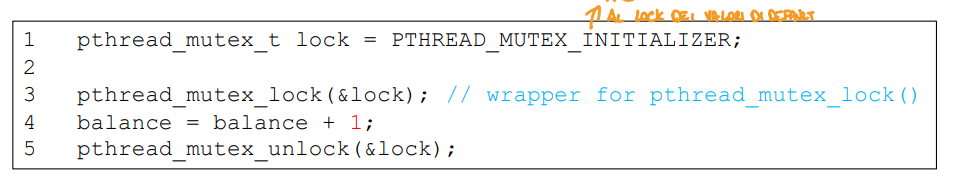
\includegraphics[width=15cm, height=3cm]{immagine_2025-01-24_122825097.png} % Percorso dell'immagine
   % \caption{Datagram Header} % Didascalia per l'immagine
    \label{fig:immagine} % Etichetta per riferimento
\end{figure}
\noindent
\subsubsection{Metriche per la valutazione dell'implementazione dei lock}
\textbf{Mutua Esclusione}: ci dice se il lock sta funzionando, se non c'è mutua esclusione il lock è inutile.\\
\textbf{Fairness (equità)}: i thread che si stanno contendendo per il lock, hanno tutti la stessa possibilità di acquisirlo?\\
\textbf{Performance}: Qual è l'overhead aggiunto per usare il lock?\\
\subsubsection{Forme di lock}
\begin{figure}[H] % Usa 'H' per forzare la posizione qui
    \centering % Centra l'immagine
    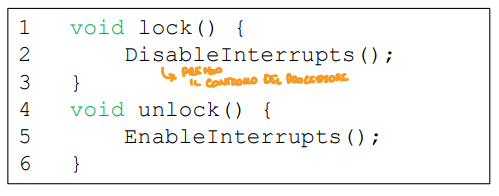
\includegraphics[width=8cm, height=3cm]{immagine_2025-01-24_123911966.png} % Percorso dell'immagine
   % \caption{Datagram Header} % Didascalia per l'immagine
    \label{fig:immagine} % Etichetta per riferimento
\end{figure}
\noindent
Problemi: richiede troppa fiducia nelle applicazioni, non funziona con i multiprocessori, perdere gl'interrupt porterebbe a seri problemi.
\begin{figure}[H] % Usa 'H' per forzare la posizione qui
    \centering % Centra l'immagine
    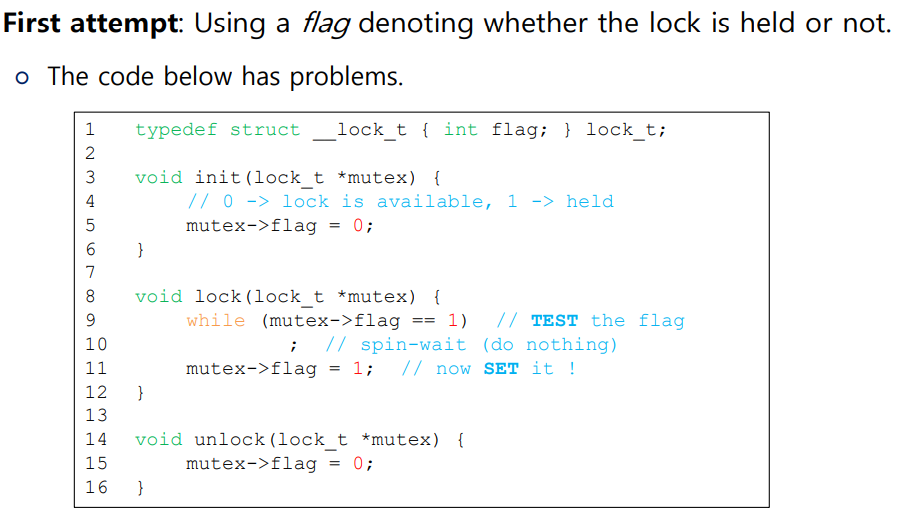
\includegraphics[width=15cm, height=10cm]{immagine_2025-01-24_124106800.png} % Percorso dell'immagine
   % \caption{Datagram Header} % Didascalia per l'immagine
    \label{fig:immagine} % Etichetta per riferimento
\end{figure}
\noindent
\begin{figure}[H] % Usa 'H' per forzare la posizione qui
    \centering % Centra l'immagine
    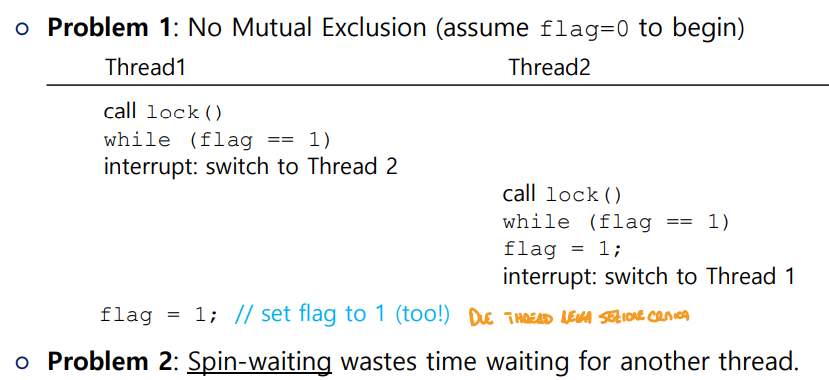
\includegraphics[width=15cm, height=8cm]{Screenshot 2025-01-24 124549.png} % Percorso dell'immagine
   % \caption{Datagram Header} % Didascalia per l'immagine
    \label{fig:immagine} % Etichetta per riferimento
\end{figure}
\noindent
Servono quindi delle istruzioni atomiche supportate dall'hardware. Come \textbf{Test and Set}.
\begin{figure}[H] % Usa 'H' per forzare la posizione qui
    \centering % Centra l'immagine
    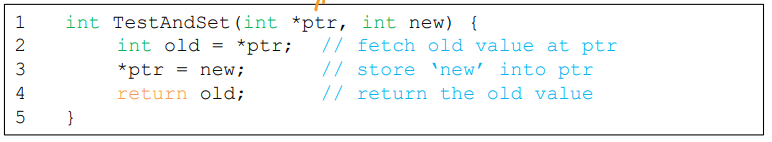
\includegraphics[width=15cm, height=3cm]{immagine_2025-01-24_124801669.png} % Percorso dell'immagine
   % \caption{Datagram Header} % Didascalia per l'immagine
    \label{fig:immagine} % Etichetta per riferimento
\end{figure}
\noindent
Questa sequenza di istruzioni viene eseguita atomicamente. Prende due parametri, un puntatore a un intero in memoria e un nuovo valore intero. Ne abbiamo visto l'implementazione con spin-lock, il problema è che non è un metodo equo.\\
\textbf{Fetch and Add} incrementa un valore atomicamente mentre ritorna il vecchio valore a un particolare indirizzo.
\begin{figure}[H] % Usa 'H' per forzare la posizione qui
    \centering % Centra l'immagine
    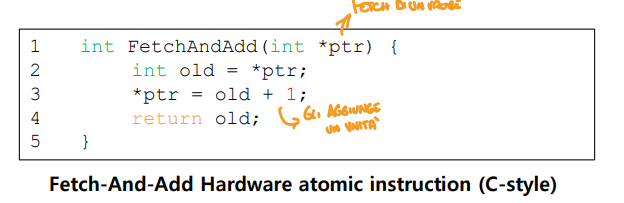
\includegraphics[width=15cm, height=3cm]{Screenshot 2025-01-24 125427.png} % Percorso dell'immagine
   % \caption{Datagram Header} % Didascalia per l'immagine
    \label{fig:immagine} % Etichetta per riferimento
\end{figure}
\noindent
Con fetch and add si va a implementare \textbf{ticket lock}.
\begin{figure}[H] % Usa 'H' per forzare la posizione qui
    \centering % Centra l'immagine
    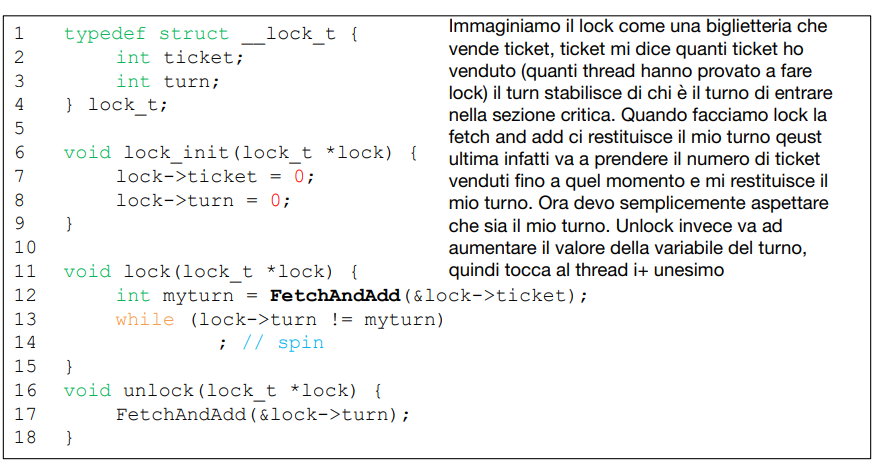
\includegraphics[width=15cm, height=9cm]{immagine_2025-01-24_125734426.png} % Percorso dell'immagine
   % \caption{Datagram Header} % Didascalia per l'immagine
    \label{fig:immagine} % Etichetta per riferimento
\end{figure}
\noindent
In alcuni casi queste soluzioni possono essere inefficienti. Quando un thread inizia ad aspettare, potrebbe sprecare un intero quanto di tempo a aspettare e controllare il valore. Per evitare lo spinning abbiamo bisogno dell aiuto del sistema operativo.
\begin{figure}[H] % Usa 'H' per forzare la posizione qui
    \centering % Centra l'immagine
    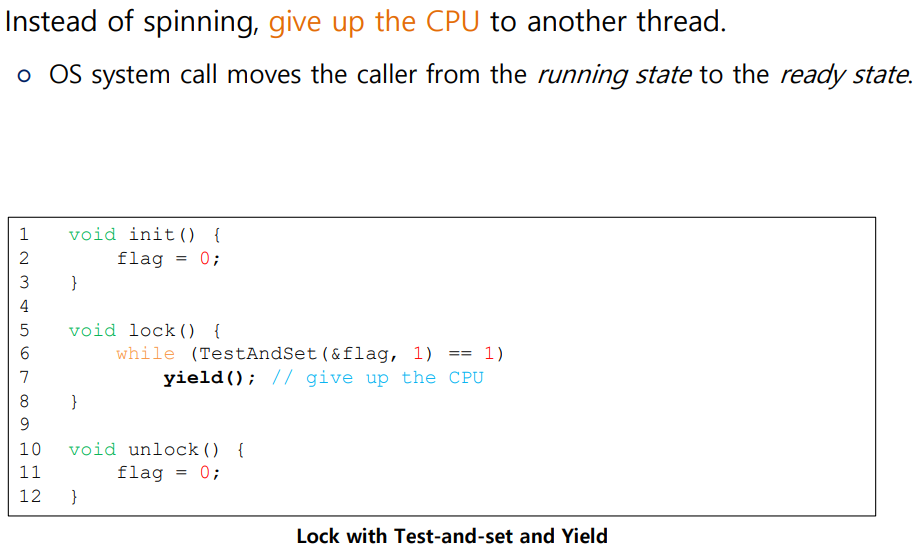
\includegraphics[width=15cm, height=9cm]{immagine_2025-01-24_125948463.png} % Percorso dell'immagine
   % \caption{Datagram Header} % Didascalia per l'immagine
    \label{fig:immagine} % Etichetta per riferimento
\end{figure}
\noindent
\end{document}
